\label{chpt:design}

Libraries such as Embree, introduced in Section~\ref{sec:embree}, provide 
optimized ray tracing algorithms that exploit parallelism on a single machine.  
When we look at larger graphics scenes that do not fit into the memory of a 
single machine, we may consider the use of distributed systems, introduced in
Section~\ref{sec:computing}, to render images.  The next generation of 
distributed systems capable of exascale computation provides an opportunity and 
in some cases a necessity to redesign current distributed applications.  Two of 
the main differences that will set exascale systems apart from current 
distributed systems are the increase in the number of nodes available and the 
reduction of the memory available per node.  For algorithm designers, this means 
there will be increased communication overhead as information will need to be
passed more frequently between individual nodes.

Communication-avoiding algorithms have been proposed as a way to reduce 
communication overhead.  The basic idea is to re-do computation instead of 
communicating results.  We use this idea as a basis for designing a distributed 
ray tracing application.  Using an optimized on-node kernel library, such as
Embree, leaves us with the key challenge of how to reduce or eliminate the
communication necessary between the nodes of the distributed system.

\section{Scene Decomposition}
\label{sec:scene_decomposition}
Designing a ray tracer for exascale systems becomes an interesting problem once
we consider scenes to render that cannot be run on a single compute node.   In
these scenes some type of decomposition to divide the scene into smaller
pieces to distribute amongst the available nodes is necessary.  To fully utilize
the on-node parallelism we would want each node to have just enough information
to fill the available memory. As each scene to be rendered is unique, the
idealized distribution for one scene will not be the same as the idealized
distribution for another.  Load balancing, a technique introduced in
Section~\ref{sec:ray_tracing}, is often used to split the scene into
equally-sized subsets.

Load balancing is often accomplished using a pre-processing step where the scene 
is optimally divided into evenly-sized subsets before ray tracing the 
scene.  As the pre-processing step is often computationally expensive, the 
expense must be considered and weighed against alternative designs. For example, 
a na\"{i}ve alternative approach is to divide the space based on a uniform 
spatial distribution.  Figure~\ref{fig:decompose-scene} presents pseudocode
for one such algorithm.  This algorithm results in unevenly balanced subsets but
takes little time to compute.  In this na\"{i}ve approach, where the scene has
not been balanced it is likely to end up with nodes that have lots of work
while other nodes have little work.

\begin{figure}[!htb]
\begin{algorithm}
decompose_scene(scene)
  out: filled voxel subsets of scene
  voxels = create_spatially_uniform_voxels()
  for each voxel in voxels do
    for each primitive in scene do
      if is_in(primitive, voxel) then
        add(voxel, primitive)
      end if
    end for
  end for
return voxels
\end{algorithm}
\caption{Pseudocode - Decompose Scene}
\label{fig:decompose-scene}
\end{figure}

Determining the optimal design pattern for scene decomposition becomes a
question of whether the cost of pre-processing outweighs the cost of an unbalanced 
system.  Assuming the pre-processing step were free, computationally speaking, 
the solution would be to use it.  This would ensure the minimum number of
nodes are used and that each one is used to its full potential, memory wise.  
However since there is a cost to pre-processing we must consider algorithms that
reduce this cost.  

Dividing the scene uniformly in space reduces the pre-processing cost, but 
potentially increases the number of required nodes.  In addition, each node may 
or may not fill the memory available.  Since each node need not be responsible 
for a single subset of the scene, it is possible to offset this concern and 
increase memory usage per node by assigning each node multiple subsets.

\begin{figure}[!htb]
\centering
\noindent\makebox[\textwidth]{%
  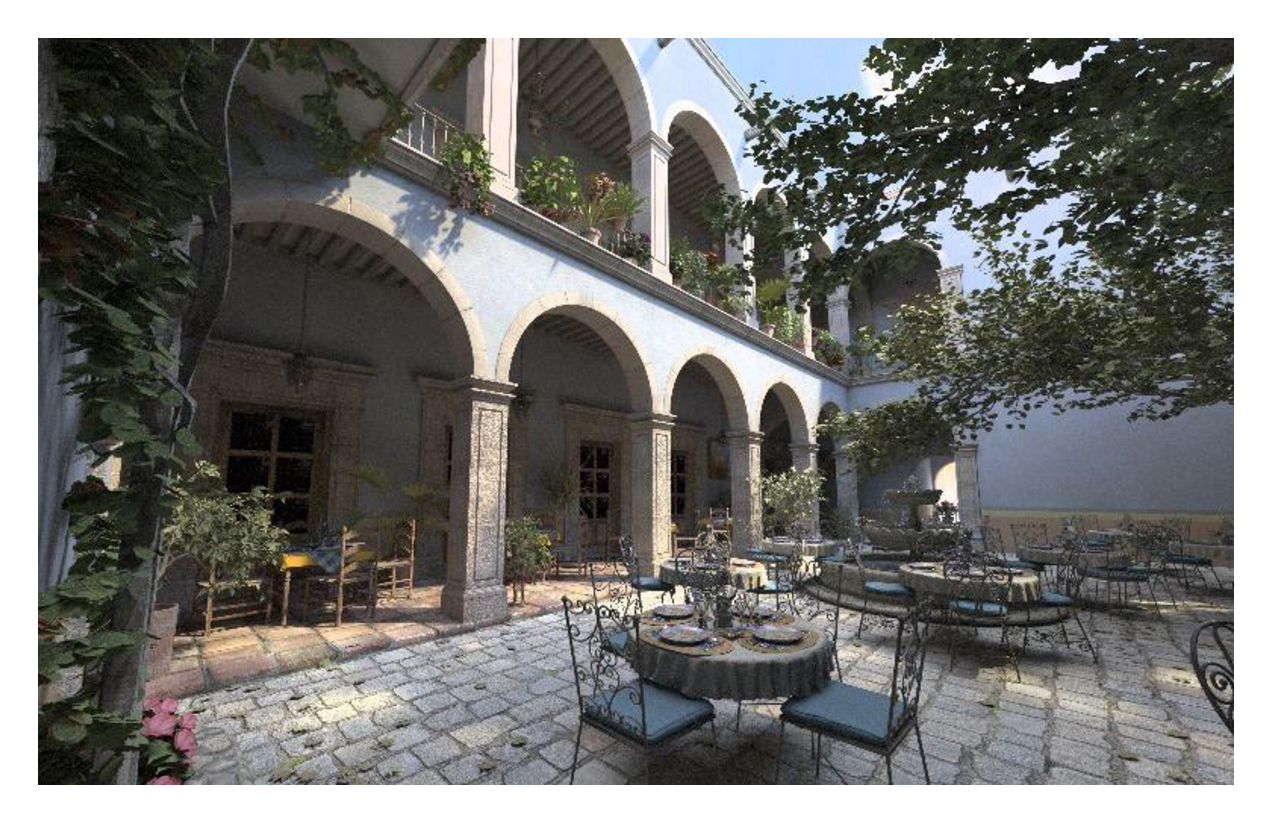
\includegraphics[height=6cm]{drawings/sanmiguel_cam25.pdf}%
  }
\caption{Example - San Miguel Scene}
\label{fig:san_miguel}
\end{figure}

As an example we will consider the San Miguel scene in
Figure~\ref{fig:san_miguel}~\cite{san-miguel-image}.  The scene was modeled by 
Guillermo M. Leal Llaguno and is based on a hacienda located in San Miguel de 
Allende, Mexico.  It is a large scene with 10,500,550 triangles and a
non-uniform distribution of information.  If we decompose the scene into 27
($=$3$\times$3$\times$3) equally-sized subsets the distribution of triangles is
shown in Figure~\ref{fig:san_miguel_scene}a is generated.  If we consider ray
tracing this scene on a machine with eight nodes a distribution such as that shown in 
Figure~\ref{fig:san_miguel_scene}b, which was generated by inspection, is
possible.  This roughly distributes the scene evenly between the nodes and
aligns neighboring subsets on the same node. If our algorithm can achieve this
type of distribution we would have a setup similar to what a more computationally
expensive pre-processing step designed to optimally distribute the scene may
compute.  As mentioned in Section~\ref{sec:task-based}, tuning hints can be
provided to many task-based programming models, the optimal balanced
distribution of voxels over available nodes is the type of information you 
might in such a specification file.  Given this, we use a spatially uniform
distribution algorithm and focus on reducing communication cost.

\begin{figure}[!htb]
\minipage{0.7\textwidth}
  \centering{
  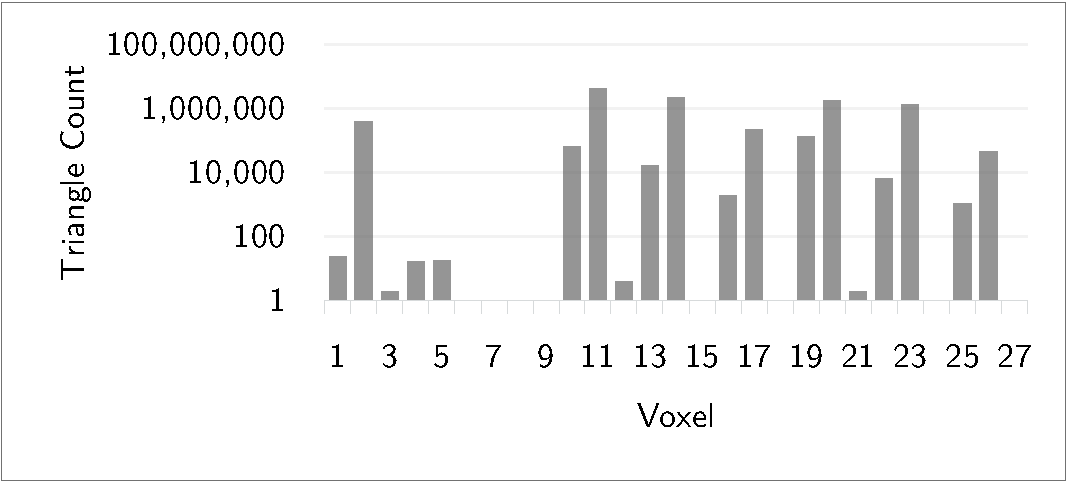
\includegraphics[width=3.5in]{drawings/examples/VoxelDistribution.pdf}
  } \\
  \centering{(a) Triangles per Voxel}
  
  \centering{
  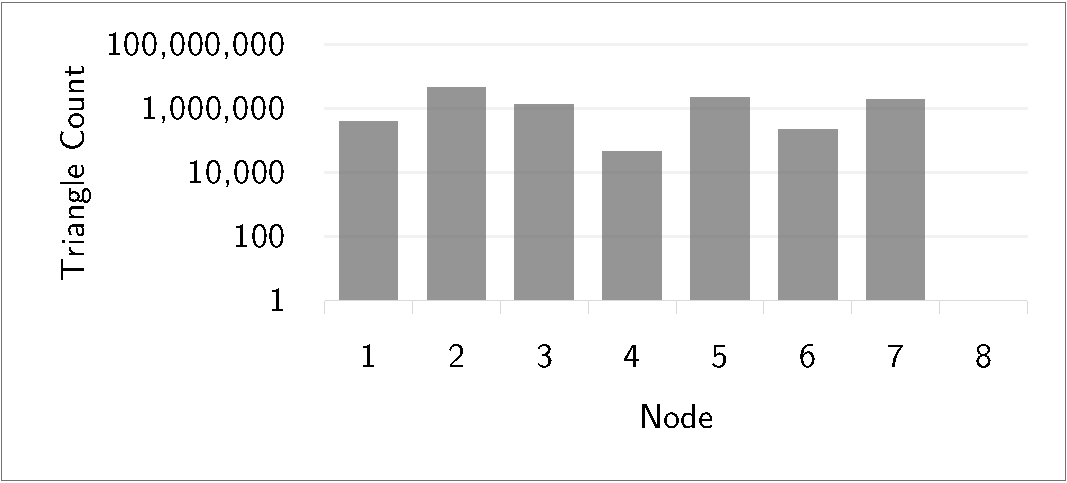
\includegraphics[width=3.5in]{drawings/examples/NodeDistribution.pdf}
  } \\
  \centering{(c) Triangles per Node}
\endminipage\hfill
\minipage{0.3\textwidth}
  \centering{
  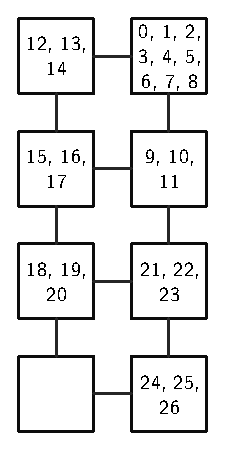
\includegraphics[width=1.5in]{drawings/examples/NodeVoxelDistribution.pdf}  
  } \\
  \centering{(b) Voxel Distribution \\ on Nodes}  
\endminipage
\caption{Example - San Miguel Voxel Decomposition}
\label{fig:san_miguel_scene}
\end{figure}


\section{Communication} 
\label{sec:communication}
Each ray cast into a scene has the potential to interact with every geometric
primitive in the scene due to reflection and refraction.  In addition, each
point being illuminated within a scene needs to cast rays towards each
luminaire.  As a result, determining which pieces of memory each ray will need
throughout the ray tracing algorithm is not a straight forward task.  With a
distributed system and in a worst-case scenario, each ray may need to
communicate with every node where subsets of the scene were distributed.

Communication is anticipated to be the bottleneck on an exascale system which
makes reducing the communication cost a high priority in our algorithm design.  
Optimally our goal is to create a ray tracing algorithm with distributed scene 
that needs little to no communication.  We explore how we might design a 
communication-avoiding ray tracer in this section.

\subsection{Communication-Avoiding Ray Casting}
\label{sec:ca-ray-casting}
To design a communication-avoiding ray tracer we will start with a simple ray
casting algorithm where only the viewing rays are traced. These rays are 
cast into a scene from the eye position.  If they hit an object, a fixed red,
green and blue, or RGB, value is set based on the object the ray intersected.
This creates a cartoon-like rendering of the scene.  Without light rays,
reflected rays and refracted rays, communication between nodes executing the
ray caster can be avoided entirely.

We can avoid all communication between nodes executing the ray casting step in a
ray casting algorithm by tracing every ray in every voxel as outlined in
Figure~\ref{fig:ray_caster}a. Each process executing over a subset of the scene,
or voxel, will receive every viewing ray as defined in
Figure~\ref{fig:ray_caster}b.  Each process then traces the rays and sets the
RGB value if the ray intersects an object in the subset of the information it
contains.

\begin{figure}[!htb]
\minipage{0.56\textwidth}
\begin{algorithm}
cast_scene(scene, camera) 
  out: a rendered image of the scene
  voxels = decompse_scene(scene)
  voxels = sort_wrt(camera, voxels)
  rays = distribute_viewing_rays(camera)
  image[rays] = false
  for each voxel in voxels do
    voxel_image = cast_voxel_rays(rays, voxel)
    for each ray in rays do
      if voxel_image[ray] then do
        image[ray] = voxel_image[ray];
      end if
    end for
  end for
return image
\end{algorithm}

\centering{(a) Cast Scene}

\endminipage\hfill
\minipage{0.4\textwidth}
\begin{algorithm}
cast_voxel_rays(rays, voxel)
  out: image, traced scene of voxel
  image[rays] = false
  for each ray in rays do
    if intersects(ray, scene) then do
      image[ray] = rgb(ray)
    end if
  end for
return image






\end{algorithm}

\centering{(b) Cast Voxel Rays}

\endminipage\hfill
\caption{Pseudocode - Ray Casting}
\label{fig:ray_caster}
\end{figure}

\begin{figure}[!h]
\centering
  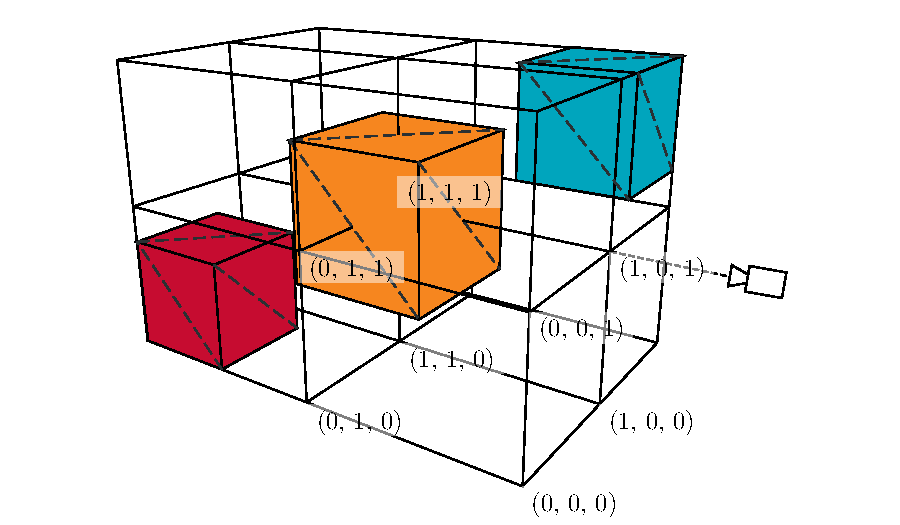
\includegraphics[width=6in]{drawings/examples/cube_example/cubes_visio.pdf}
\caption{Example - Ray Casting Cubes}
\label{fig:cubes_3d}
\end{figure}

The painters algorithm~\cite{book-shirley}, which ``paints'' pixels 
using a back-to-front voxel ordering with respect to the camera position, can
then be used to produce the final image.  This ensures the pixels from
front voxels paint over pixels from back voxels.  As an illustration we can
consider the simple scene in Figure~\ref{fig:cubes_3d} which has three cubes
placed along a diagonal.  Each cube is tessellated into twelve triangles, two
for each face.  If we distribute the scene into 8 ($=$2$\times$2$\times$2)
equally-sized voxels sharing the orange cube, one voxel with the red cube and
one voxel with the blue cube.  The voxels are indexed using the i, j, and k
coordinates of the voxel's vertex closest to the origin of the voxel grid.

If we trace an orthographic view of the scene from the camera position shown,
each voxel computation produces the corresponding images shown in
Figure~\ref{fig:cubes_example}.  The triangle geometry from the indicated voxel is
outlined for clarity. Rays that intersect the inside of an object are shown in
gray.

\begin{figure}[!htb]
\minipage{0.25\textwidth}
  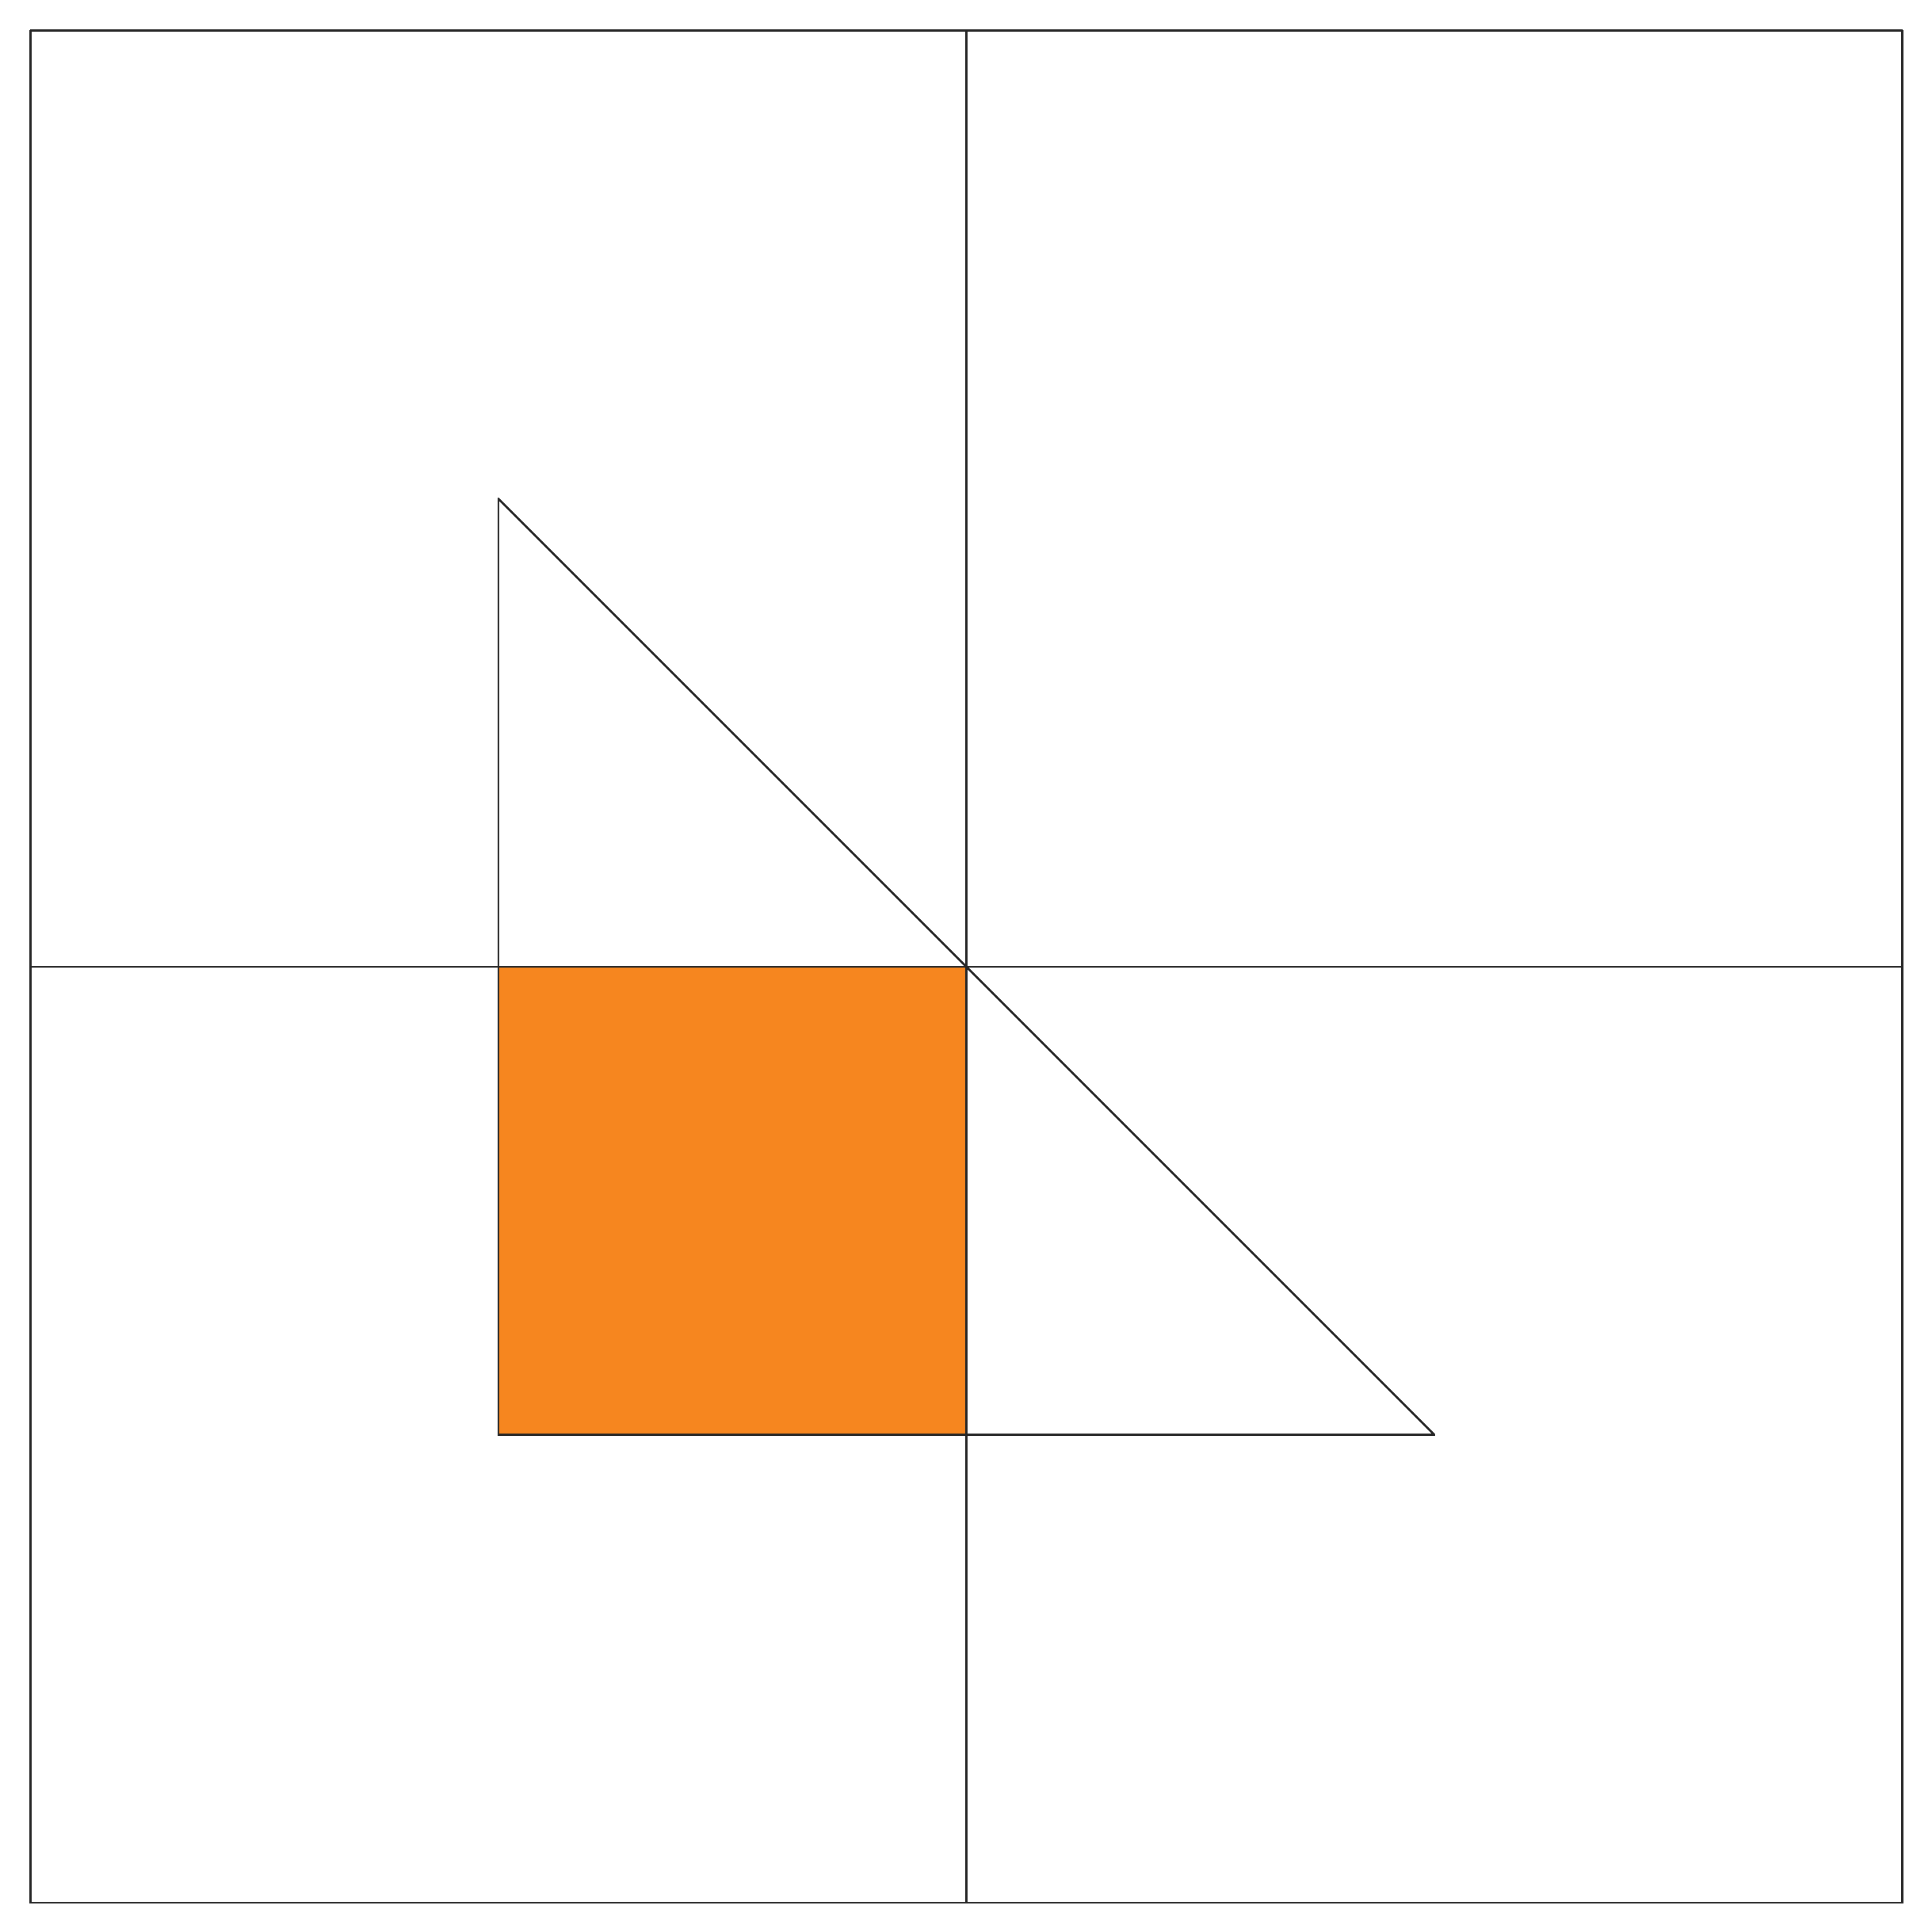
\includegraphics[width=\linewidth]{drawings/examples/cube_example/cubes_01.pdf}
  \centering{(0, 0, 0)}
  
  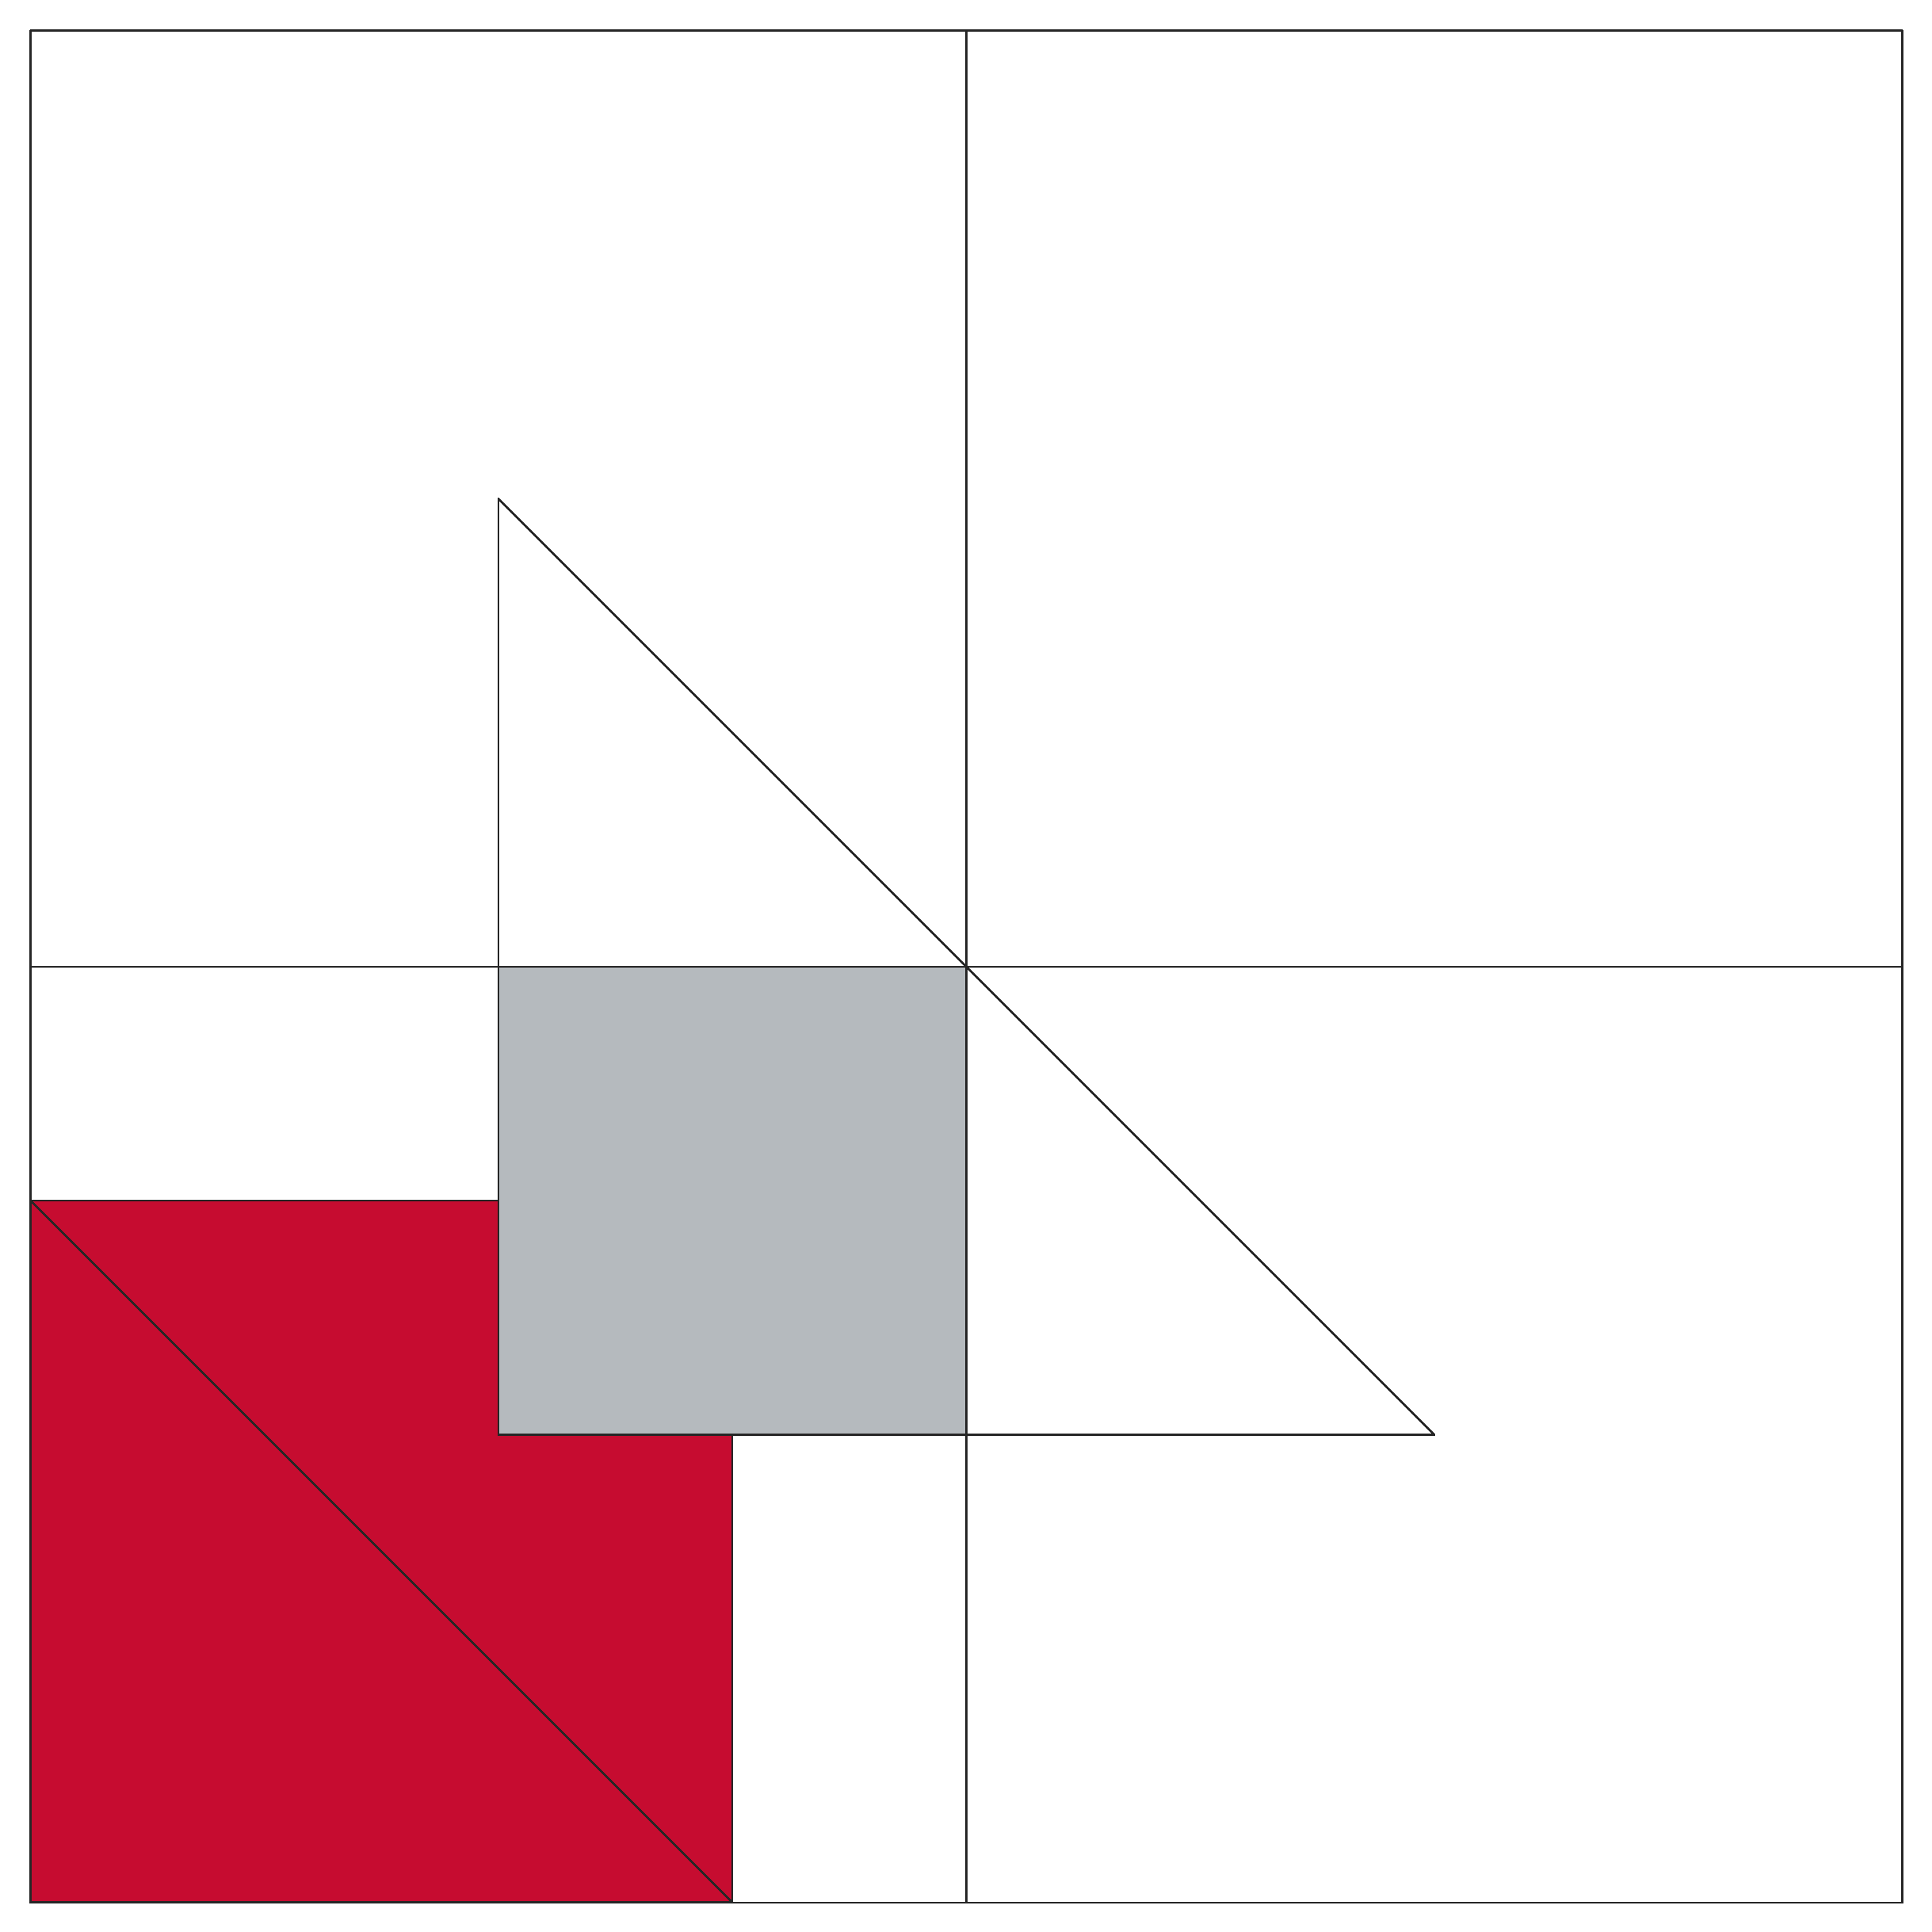
\includegraphics[width=\linewidth]{drawings/examples/cube_example/cubes_05.pdf}
  \centering{(0, 0, 1)}
\endminipage\hfill
\minipage{0.25\textwidth}
  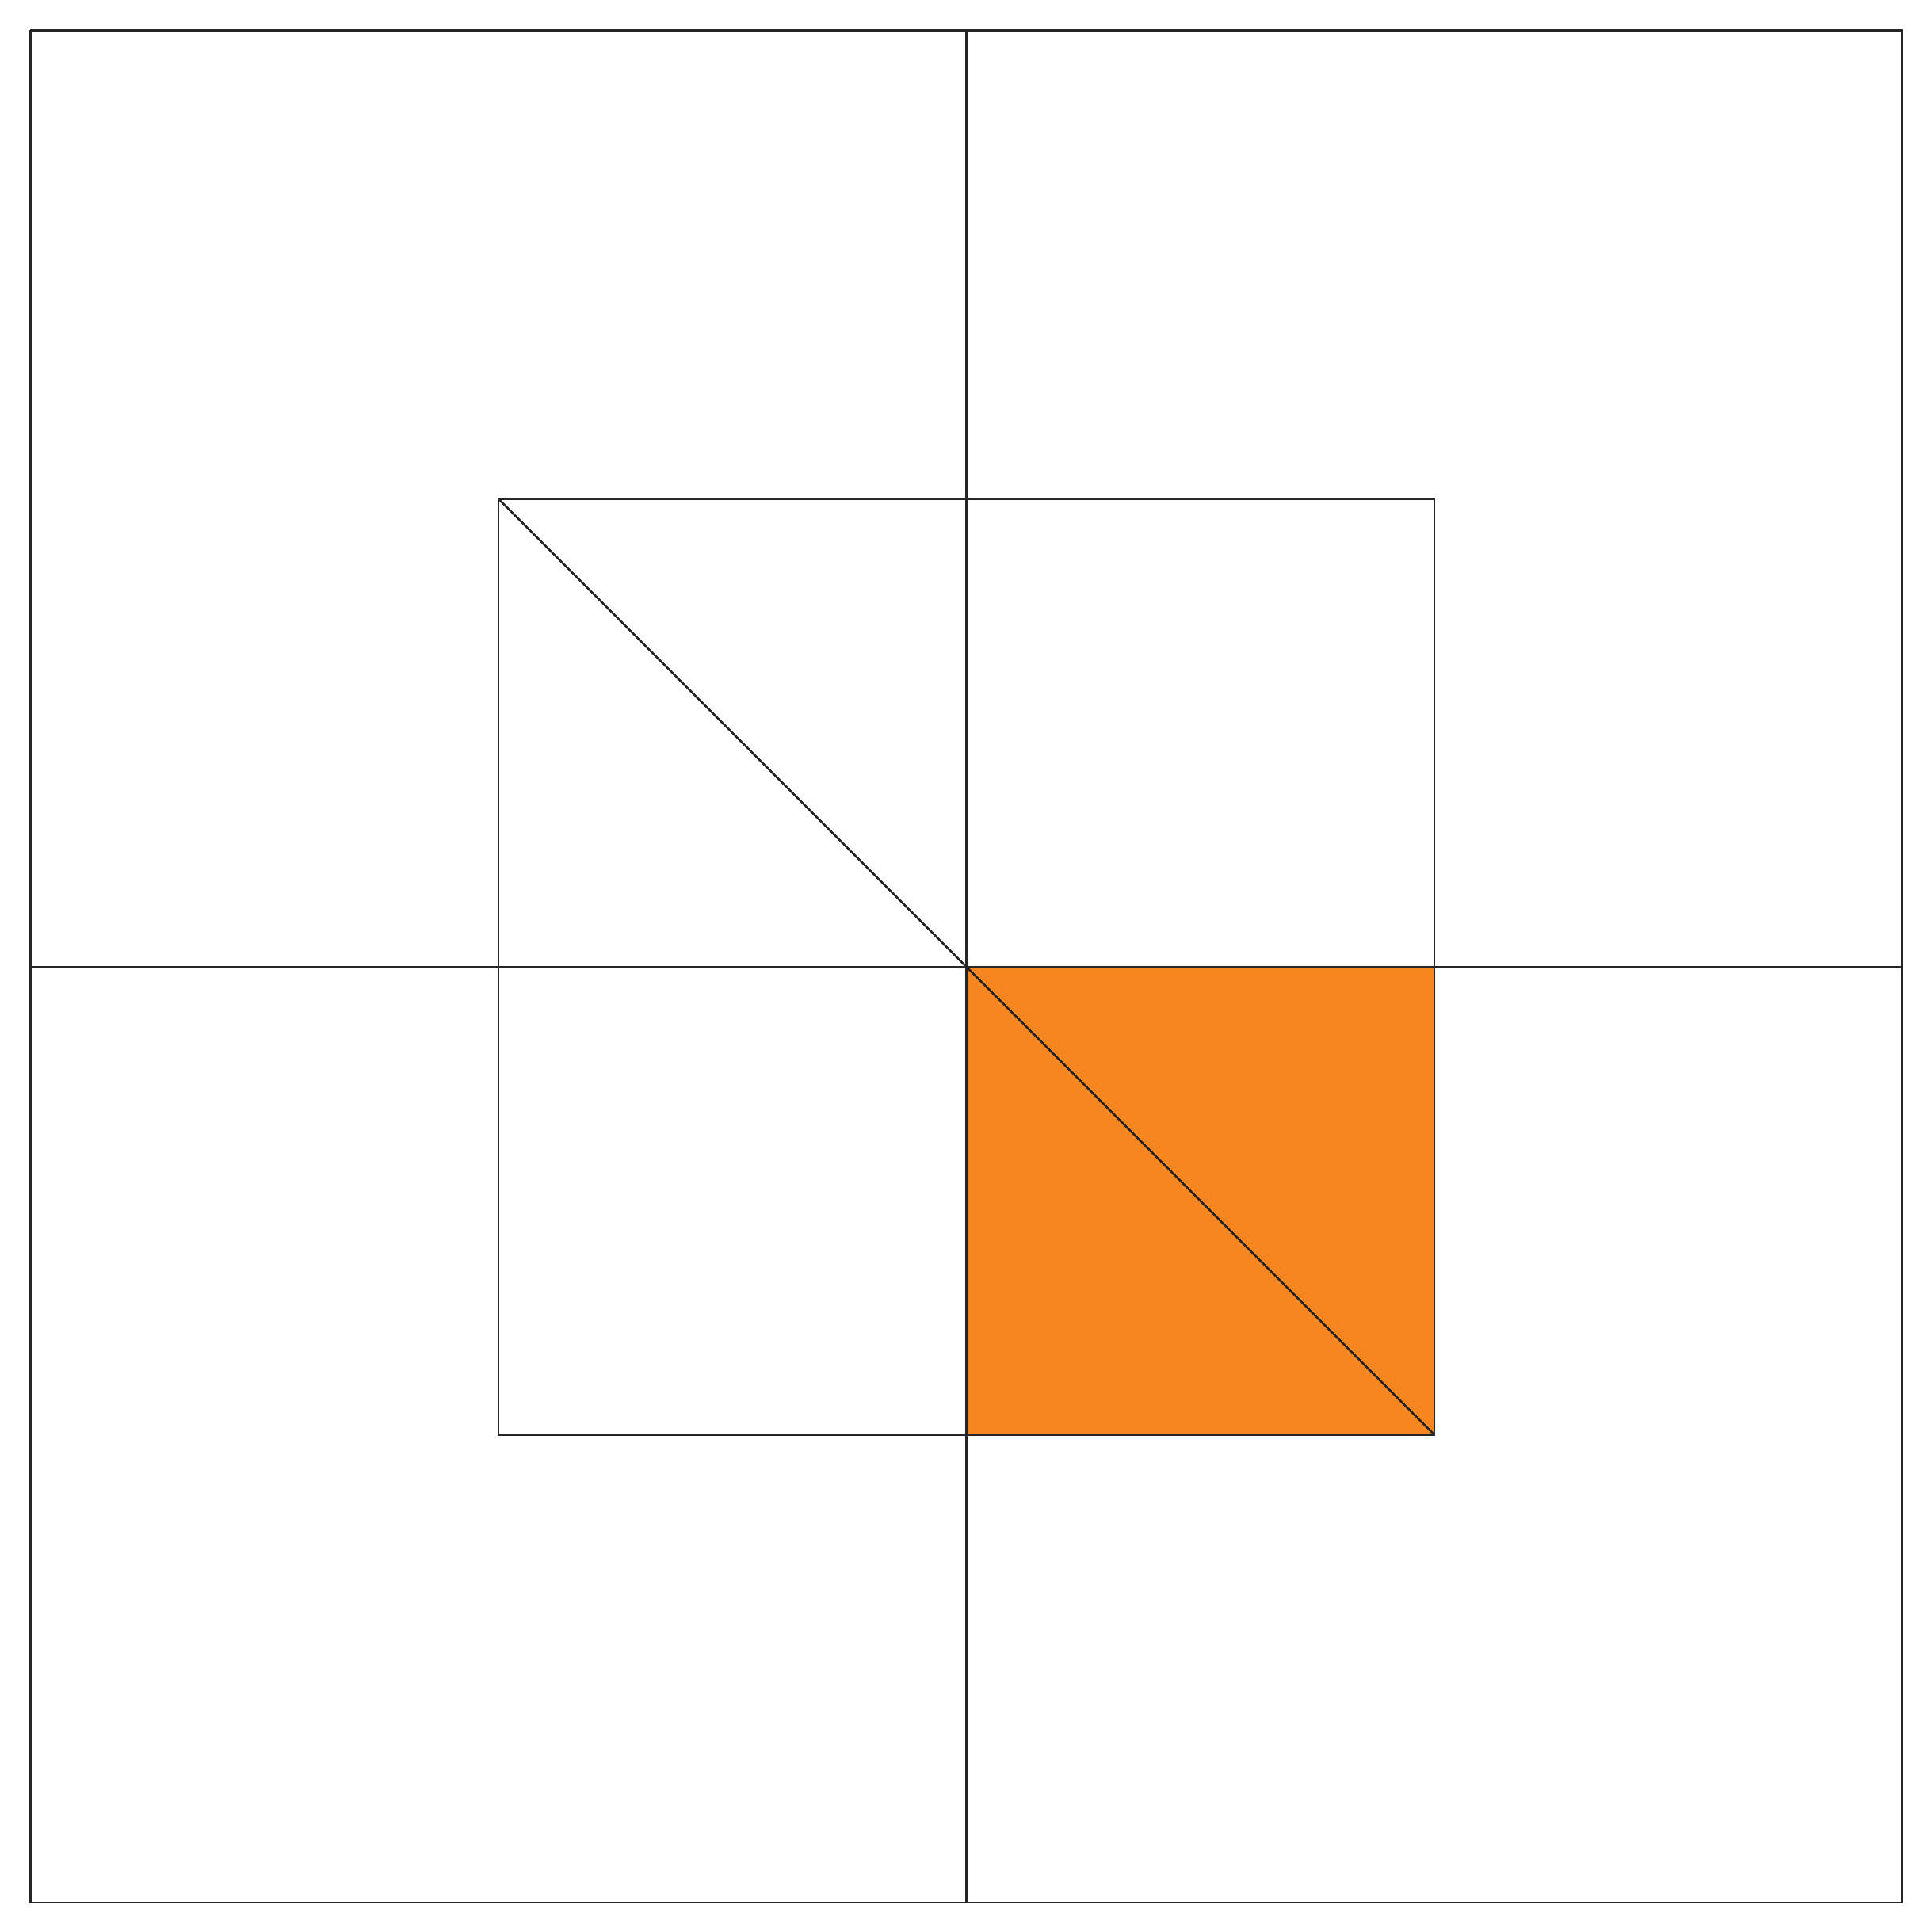
\includegraphics[width=\linewidth]{drawings/examples/cube_example/cubes_02.pdf}
  \centering{(1, 0, 0)}
  
  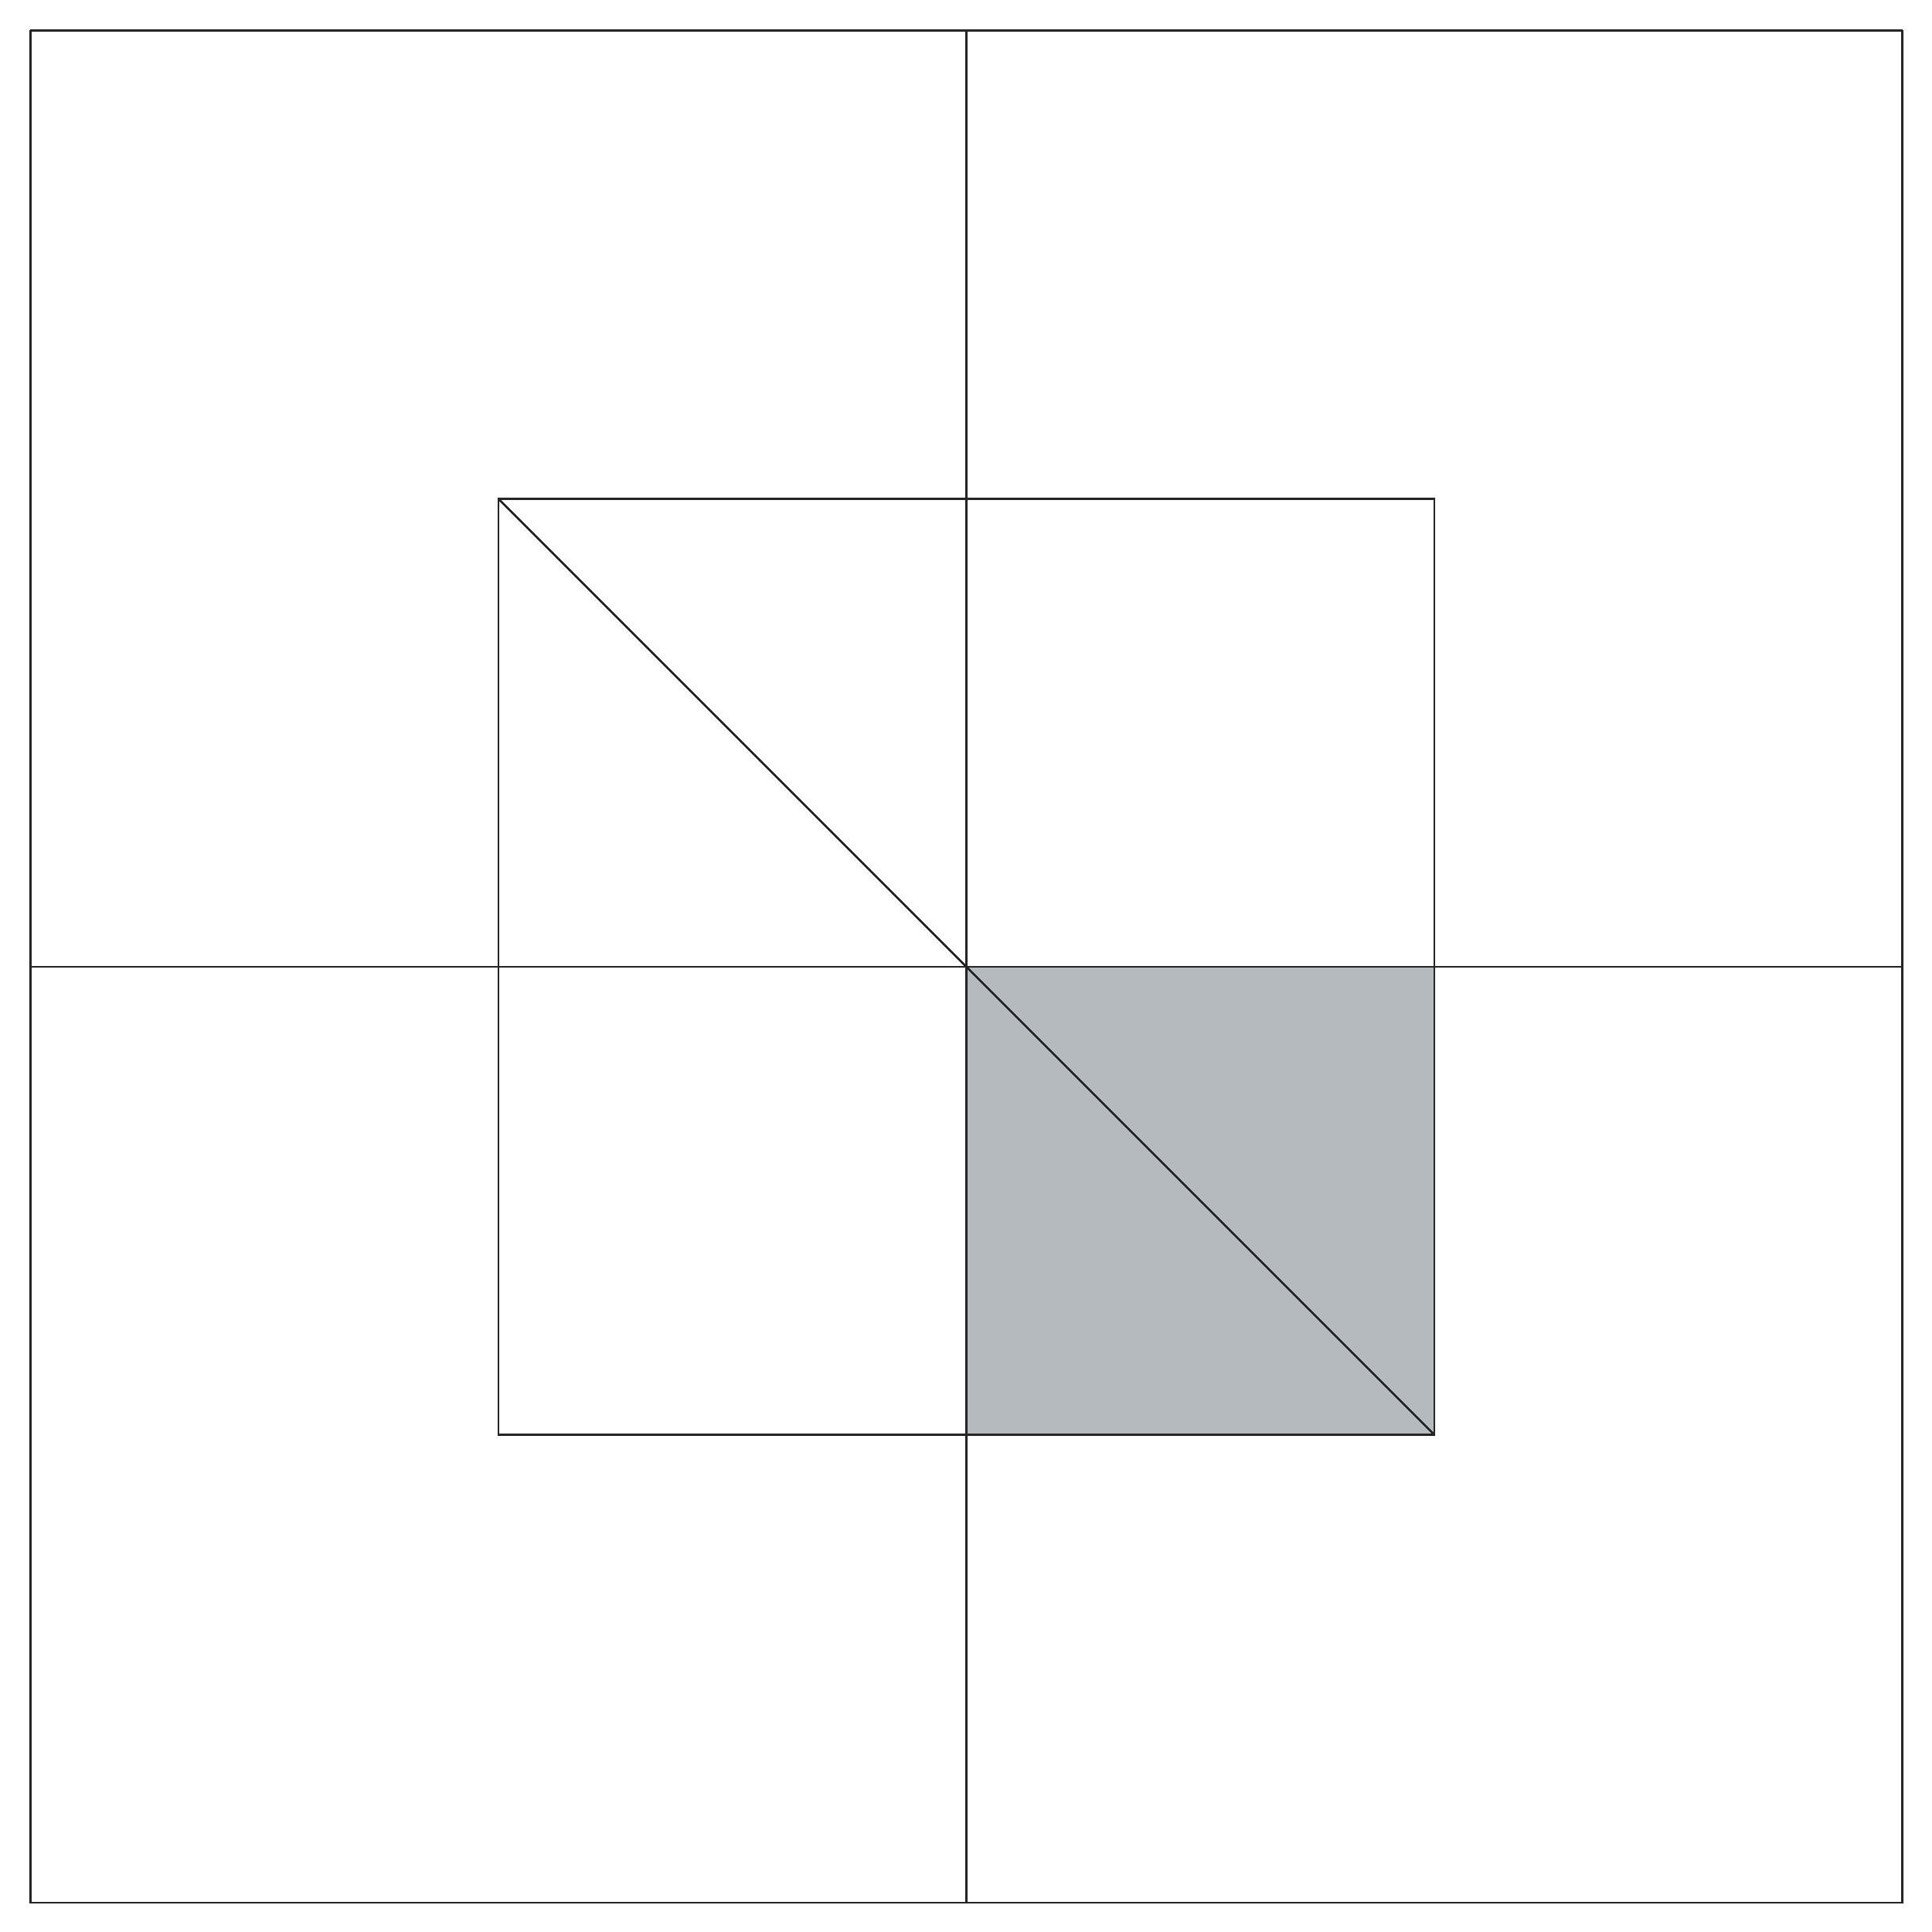
\includegraphics[width=\linewidth]{drawings/examples/cube_example/cubes_06.pdf}
  \centering{(1, 0, 1)}
\endminipage\hfill
\minipage{0.25\textwidth}%
  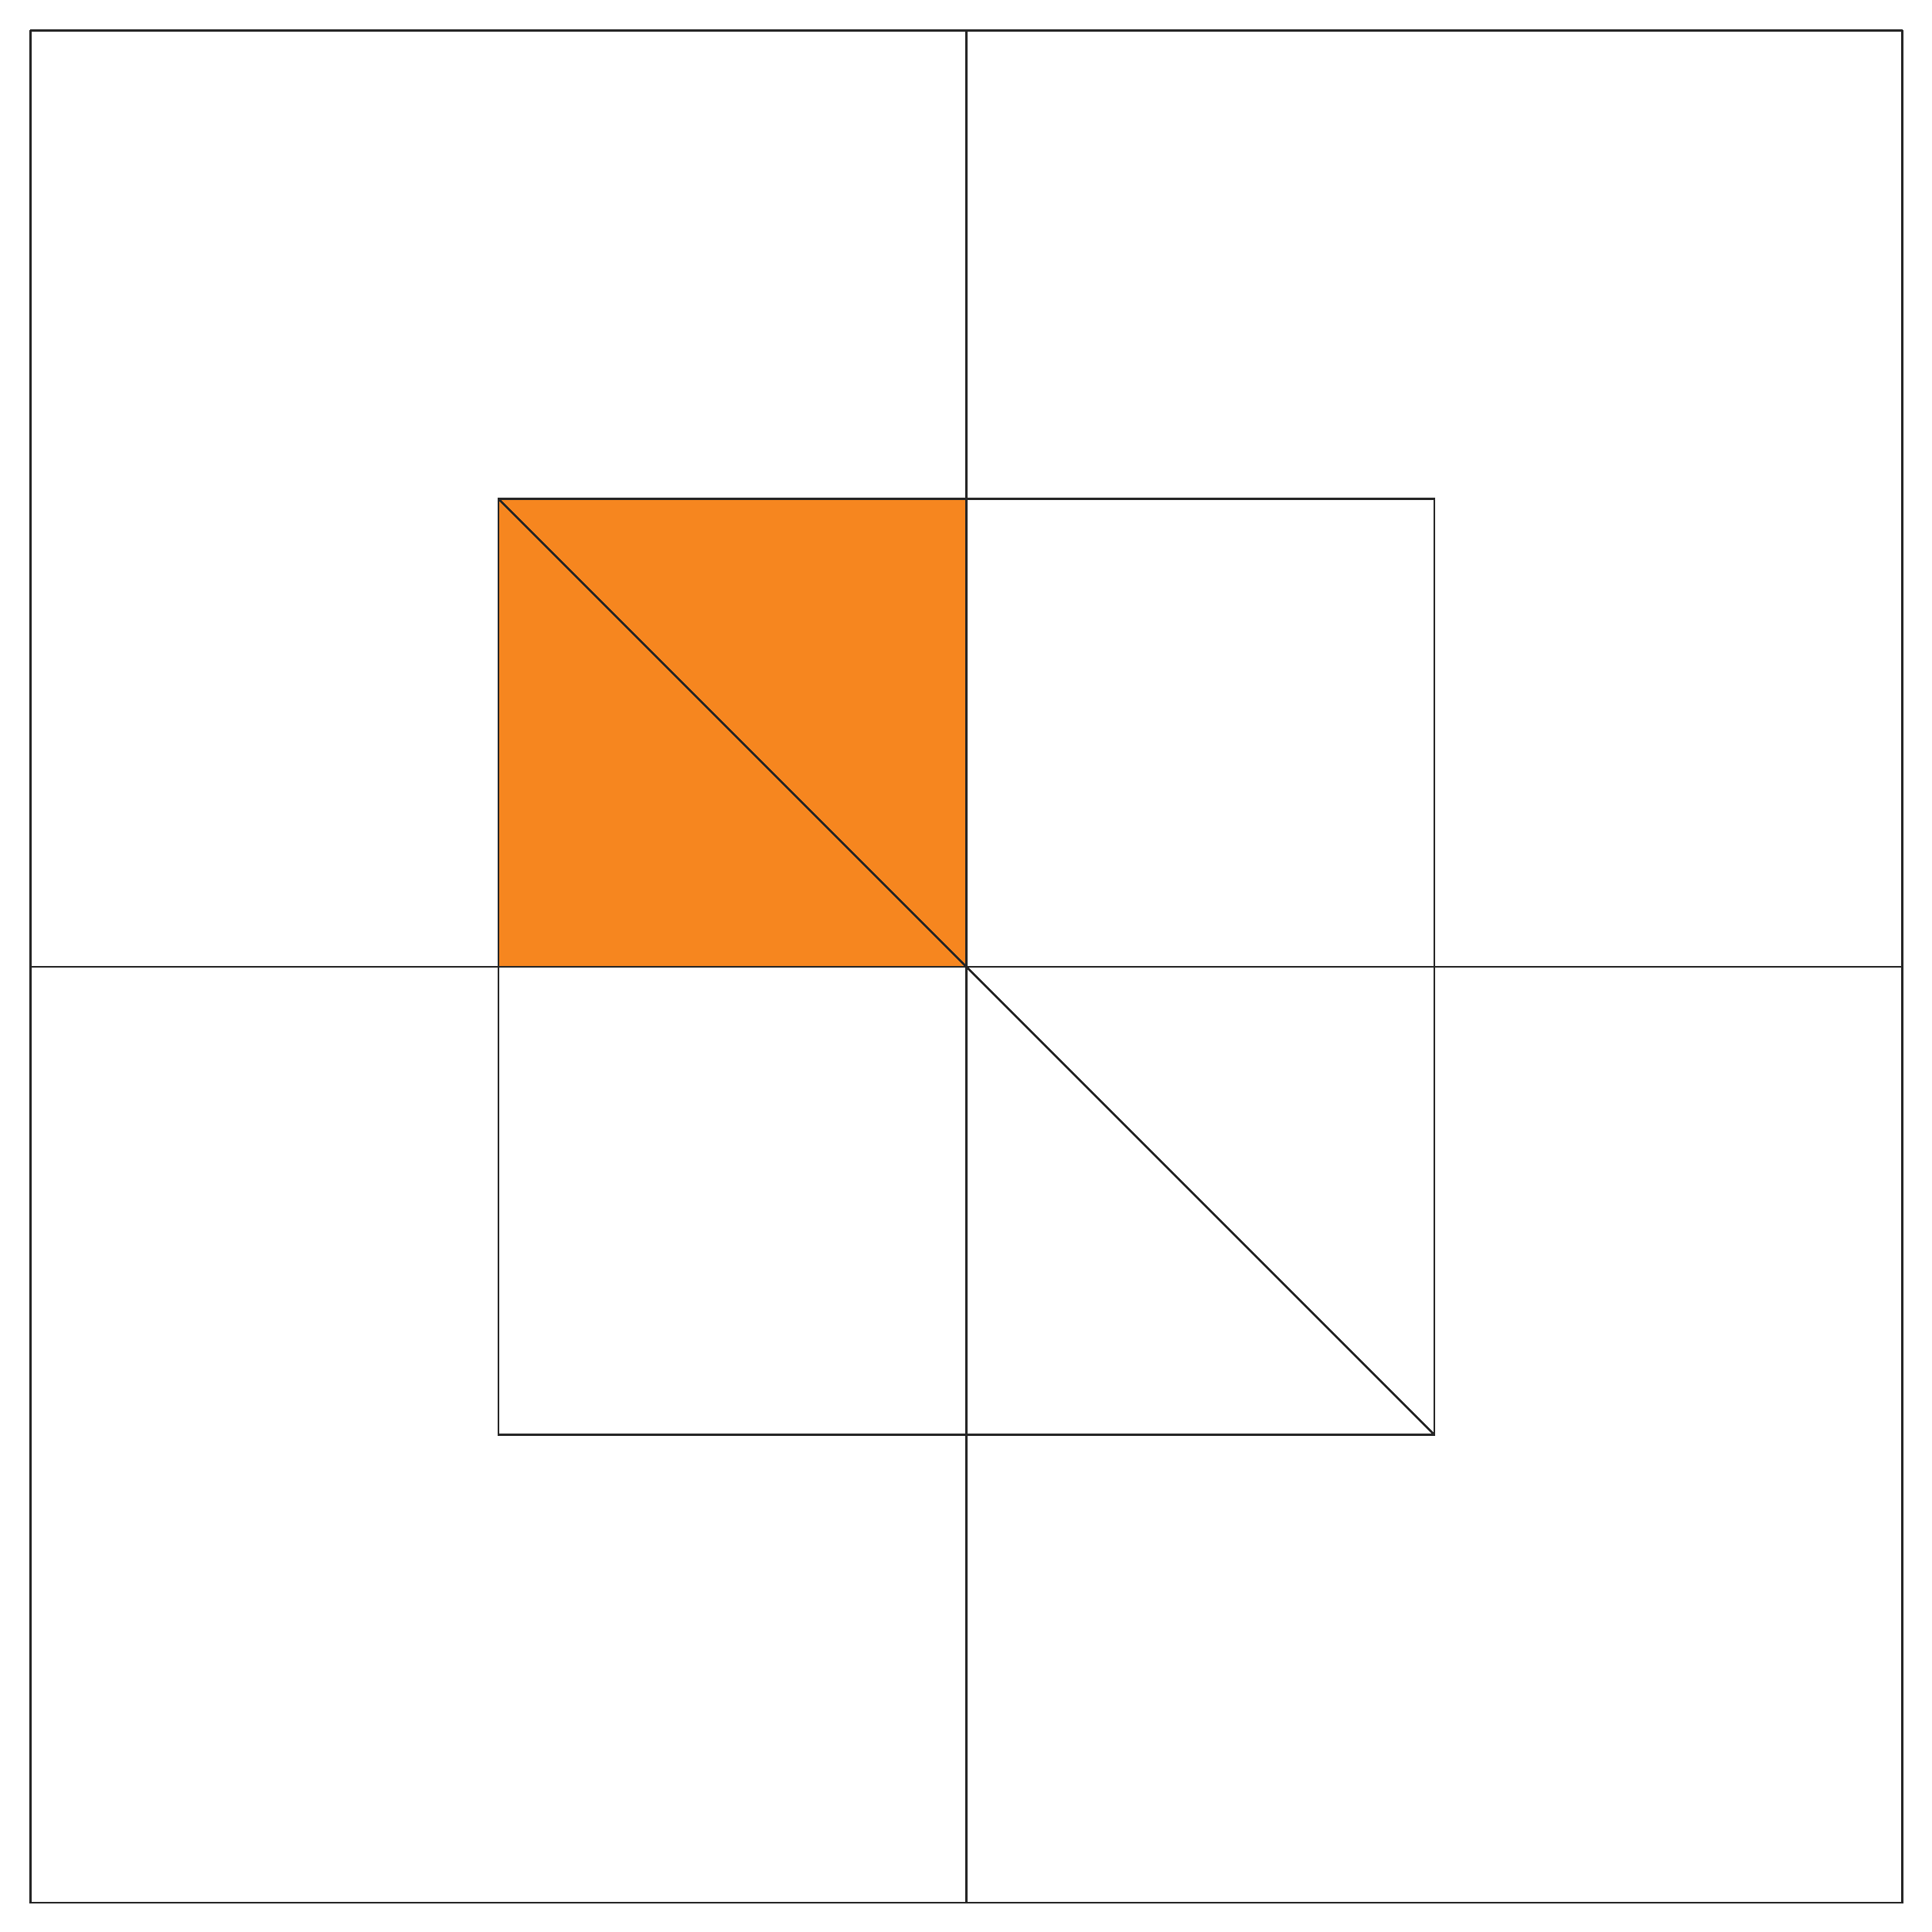
\includegraphics[width=\linewidth]{drawings/examples/cube_example/cubes_03.pdf}
  \centering{(0, 1, 0)}
  
  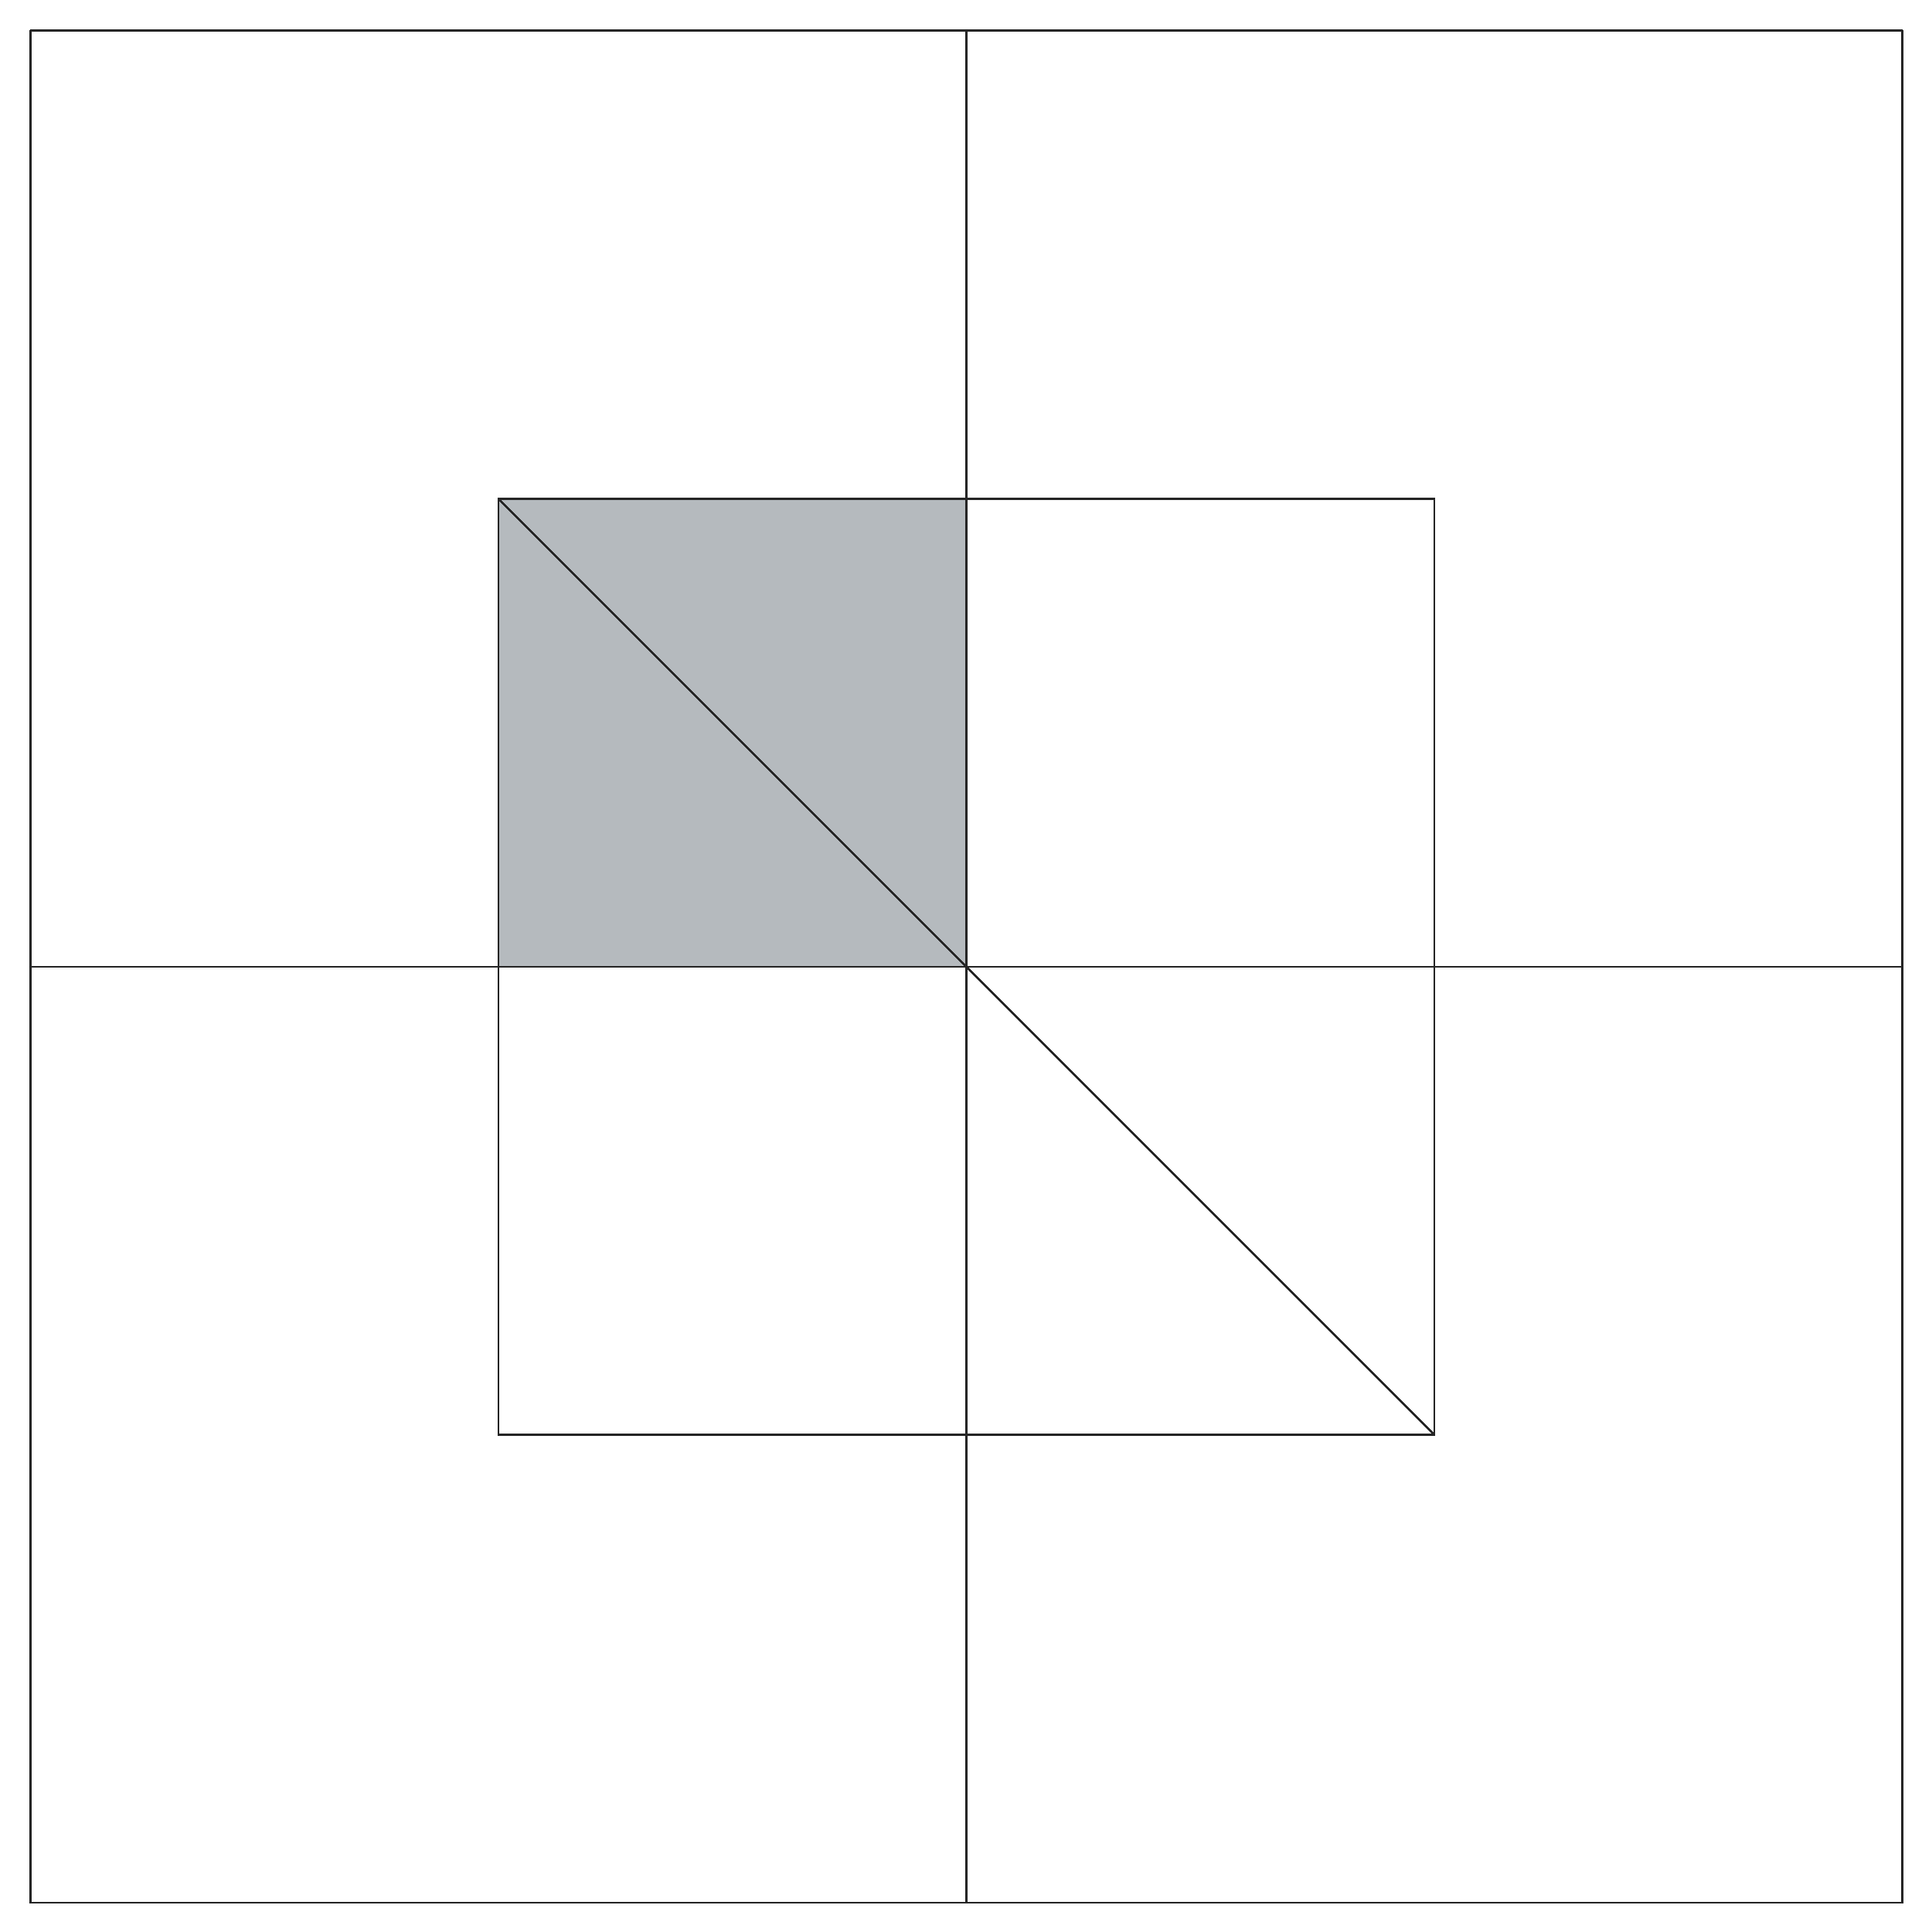
\includegraphics[width=\linewidth]{drawings/examples/cube_example/cubes_07.pdf}
  \centering{(0, 1, 1)}
\endminipage
\minipage{0.25\textwidth}%
  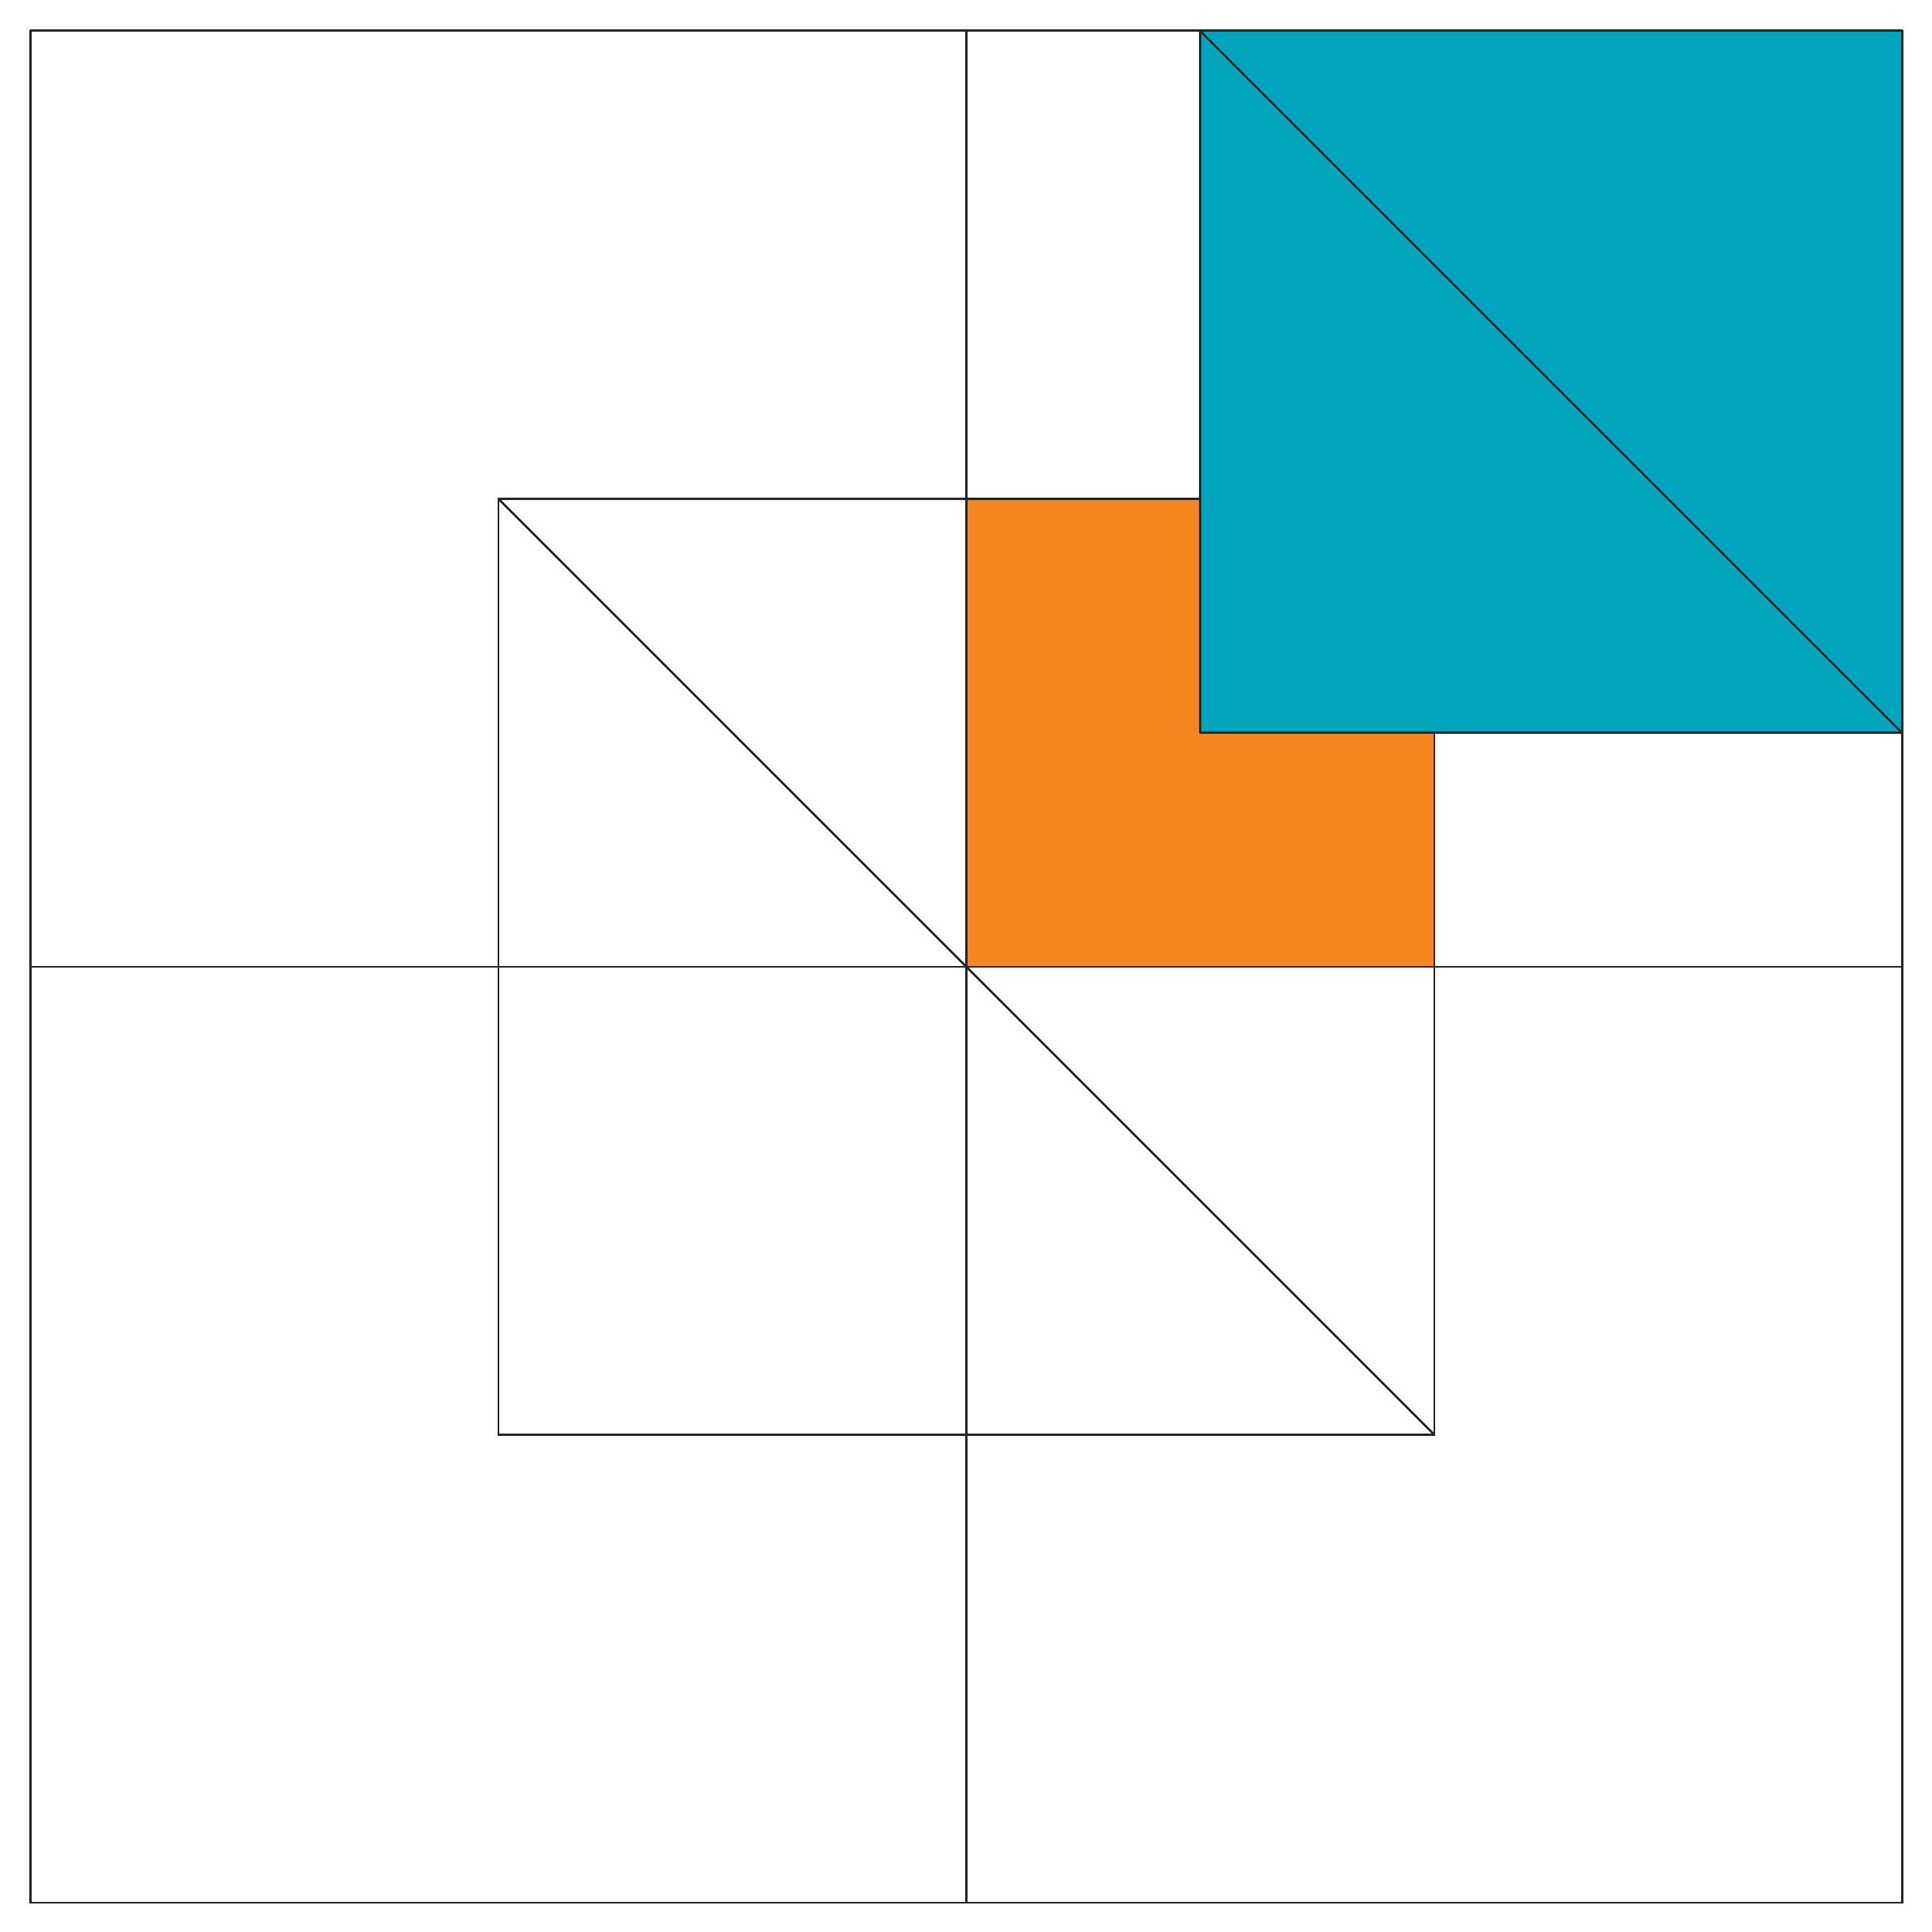
\includegraphics[width=\linewidth]{drawings/examples/cube_example/cubes_04.pdf}
  \centering{(1, 1, 0)}
  
  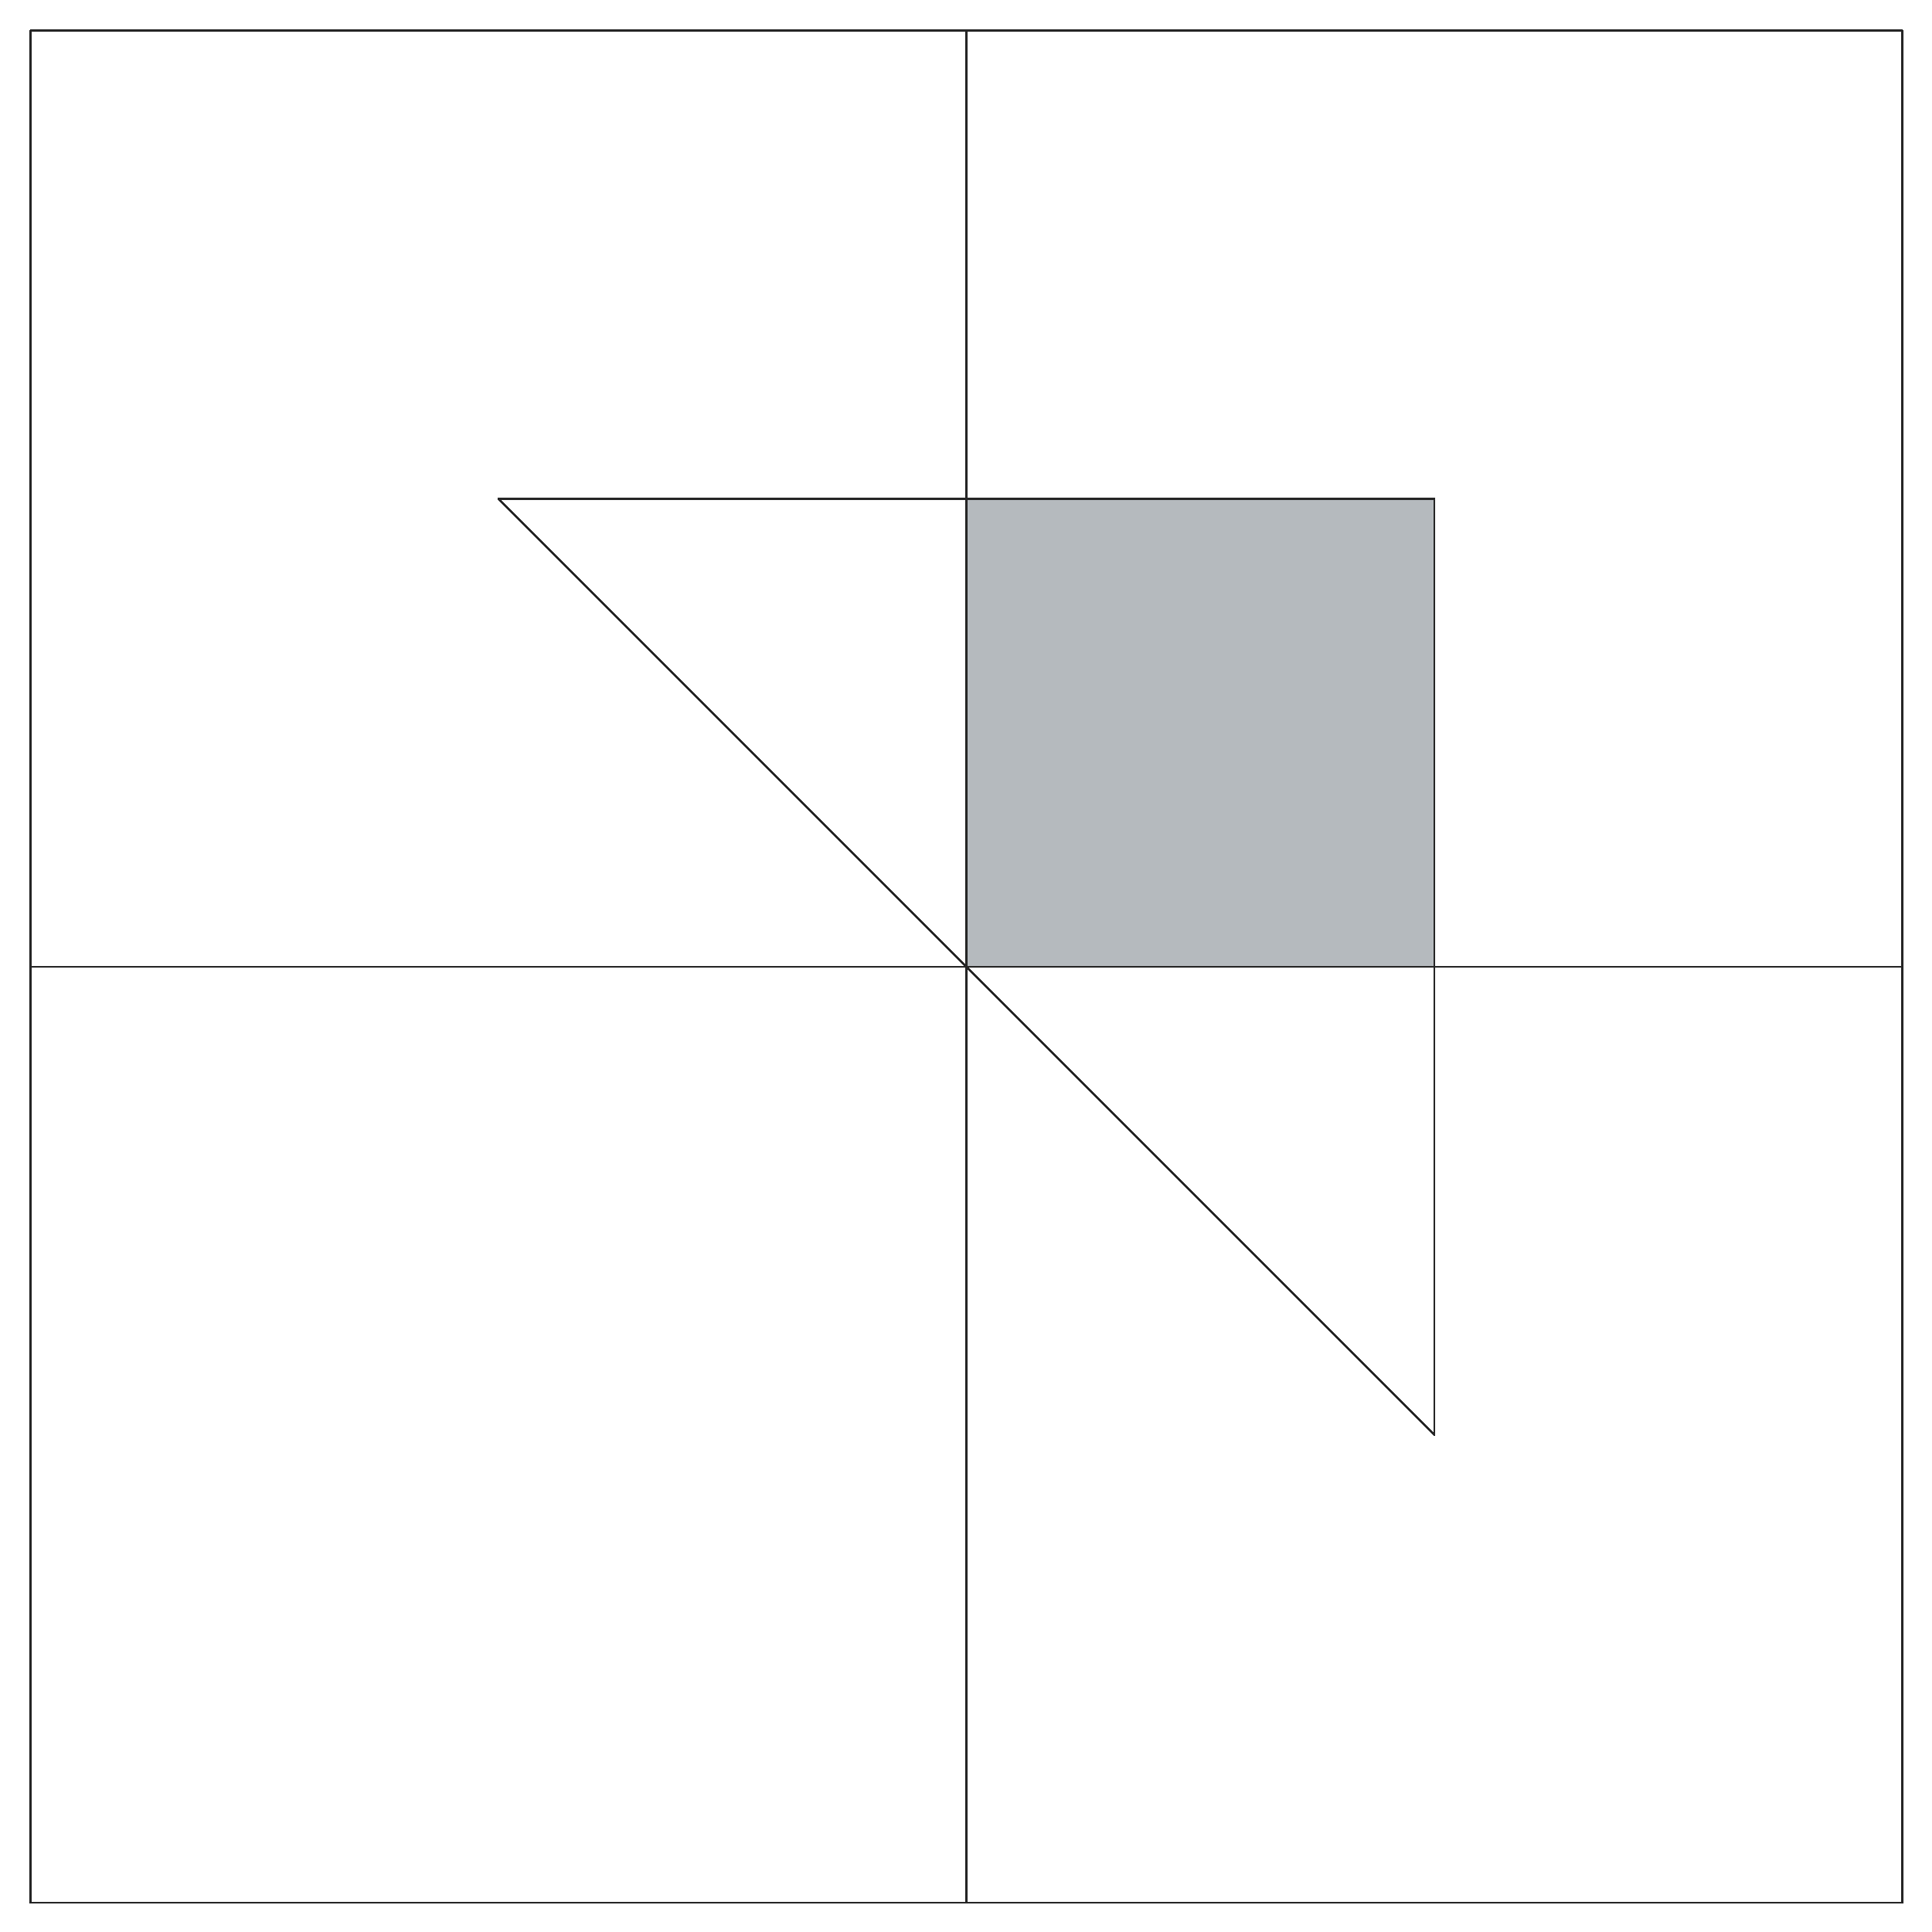
\includegraphics[width=\linewidth]{drawings/examples/cube_example/cubes_08.pdf}
  \centering{(1, 1, 1)}
\endminipage

\centering{
\includegraphics[width=.25\linewidth]{drawings/examples/cube_example/cube_final.pdf}}

\centering{Final Image}

\begin{flushleft}\caption{Example - Ray Casting Cubes - Images Produced by
Trace Voxels}{Each image shows the orthographic view of the result of rendering the
specified voxel.  The geometry contained in the voxel is outlined. 
Intersections of rays with the inside of an object are shown in gray.}
\label{fig:cubes_example}
\end{flushleft}%
\end{figure}
\subsection{Communication-Avoiding Ray Tracing}
\label{sec:ca-ray-tracing}

Expanding on the ray casting algorithm, we now look at how we might design 
similar communication-avoiding algorithms to implement shading and shadows.  
Most shading models use a second set of rays cast from an intersection point in 
the direction of each luminaire.  To compute shadows, it is important to know 
if the light rays intersect other objects in the scene anywhere along the path
from the intersection point to the luminaire.  

Casting rays from each intersection point towards each luminaire results in
a significant amount of communication if the rays pass through multiple voxels.
To eliminate this cost we introduce a technique that creates a mesh for each 
luminaire on the walls of each voxel.  The mesh, which we will call a shadow
mesh, is then traced for each voxel to determine which light rays pass through
the voxel and which are obstructed.  The shadow mesh is used by the algorithm
compiling the final image to compute the correct RGB to assign each pixel. This
concept is illustrated in Figure~\ref{fig:light-distribution} and further
explained in Section~\ref{sec:algorithm}.

\begin{figure}[!htb]
\centering
\begin{subfigure}{0.49\textwidth}
 \centering
  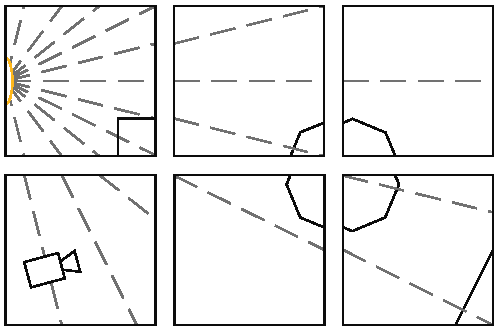
\includegraphics[width=.98\columnwidth]{drawings/examples/Lights1.pdf}
  \caption{Light Rays}
\end{subfigure}
\begin{subfigure}{0.49\textwidth}
 \centering
  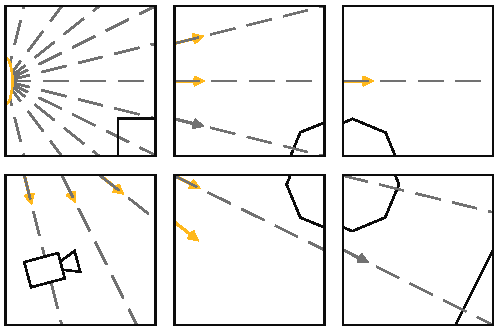
\includegraphics[width=.98\columnwidth]{drawings/examples/Lights2.pdf}
  \caption{Traced Shadow Meshes}
\end{subfigure}
\caption{Example - Shadow Mesh Generation}
\label{fig:light-distribution}
\end{figure}

\subsection{Reflection and Refraction}
The ray tracing algorithm presented in the next section supports shading,
shadows and scenes with multiple luminaires.  Although not implemented within
the scope of this thesis, we introduce a communication-avoiding strategy for
handling reflected and refracted rays in
Chapter~\ref{future-work-and-conclusions}.  Reflected rays are rays that
intersect a reflective surface and change trajectories, refracted rays change
trajectory as they pass through a surface.  The technique introduced takes a
second pass through the ray tracing algorithm to trace rays from intersection
points on reflective surfaces.  A restart capability that may exist in the
runtime systems of future exascale distributed systems is used to restart
\textbf{trace\_viewing\_rays} with the reflected or refracted rays as shown in
Figure ~\ref{fig:design}.

\newpage

\begin{figure}[!htb]
\centering
  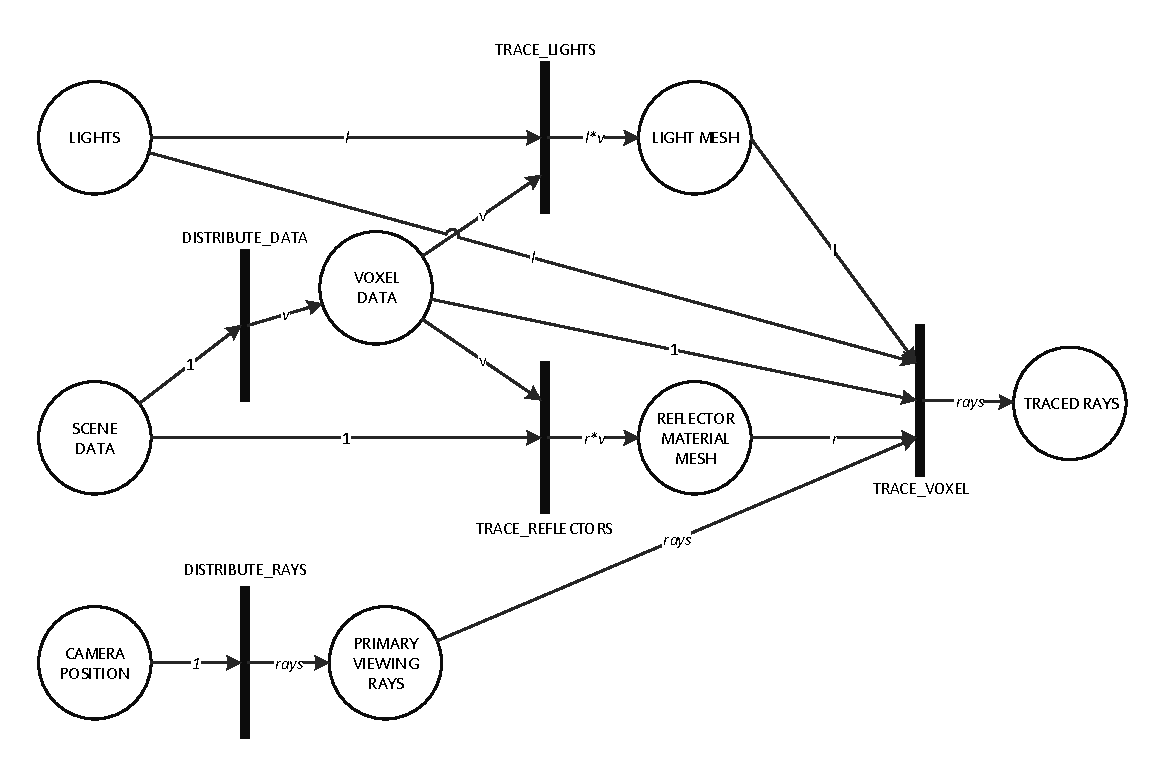
\includegraphics[width=\linewidth]{drawings/Design.pdf}
\caption{Petri Net - Ray Tracer}
\label{fig:design}
\end{figure}

\section{Ray Tracing Algorithm}
\label{sec:algorithm}
Using a spatially uniform distribution algorithm as described in 
Section~\ref{sec:scene_decomposition} and reducing communication as described in 
Section~\ref{sec:communication} allows us to design the communication-avoiding 
ray tracer outlined in Figure~\ref{fig:design}.  The figure shows a 
Petri net describing the main components of a ray tracing algorithm.  Petri 
nets are introduced in Section~\ref{sec:petri-nets}.  The following sections 
break down each place and transition.  For the scope of this thesis we have 
implemented the highlighted parts producing a ray tracer that supports shading
and shadows.  Implementation details can be found in 
Chapter~\ref{chpt:implementation}.  

\subsection{Inputs}
The required inputs for the ray tracer are lighting, camera and scene object 
properties.  There will be a single scene with potentially many luminaires.  
Multiple camera positions can be traced, but each pass through 
\textbf{trace\_viewing\_rays} will use a single camera position.  The labels 
on the arcs indicate the quantity relationships.

\subsection{Decompose Scene}
The transition \textbf{decompose\_scene} takes a \emph{scene} as input and 
produces a set of \emph{voxels} containing subsets of the scene.  Pseudo
code is presented in Figure~\ref{fig:decompose-scene}.  A geometric primitive is 
considered in a voxel if any part of the primitive falls within the voxel. This
results in geometry that crosses voxel walls being duplicated in neighboring
voxels.  The number of voxels created is represented on the arc as \emph{v}. 
For clarity we will use the term voxel to refer to an entity that contains a
subset of the scene, both geometry and material information.

\subsection{Distribute Viewing Rays}
The transition \textbf{distribute\_viewing\_rays} takes camera properties as 
input and produces \emph{viewing rays}.  The number of viewing rays in the
distribution is represented as \emph{lv}.

\subsection{Distribute Light Rays}
The transition \textbf{distribute\_light\_rays} takes a luminaire as input and 
produces \emph{light rays}.  The number of light rays in the distribution is
represented on the arc as \emph{lr}.  The distribution of light rays is
dependent on the type of luminaire being used, additional information on the
algorithm implemented can be found in
Section~\ref{sec:implementation-step-collections}.

\newpage

\begin{figure}[!htb]
\begin{algorithm}
trace_light_rays(light_rays, voxel) 
  out: shadow mesh for the luminaire and voxel
  for each light_ray in light_rays
    shadow_meshes[voxel][luminaire][light_ray] = intersects(light_ray, voxel)
  end for
return shadow_meshes
\end{algorithm}
\caption{Pseudocode - Trace Light Rays}
\label{fig:trace-light-rays}
\end{figure} 

\subsection{Trace Light Rays}
The transition \textbf{trace\_light\_rays} takes the \emph{light rays} 
distributed from a luminaire and a \emph{voxel} as input and produces a 
\emph{shadow mesh}.  The shadow mesh contains a boolean value for each light ray 
indicating whether or not the ray hit an object in the voxel being traced.  
Pseudocode is presented in Figure~\ref{fig:trace-light-rays}. 

\begin{figure}[!htb]
\begin{algorithm}
trace_viewing_rays(viewing_rays, luminaires, voxel) 
  out: traced images for the voxel, one for each luminaire
  traced_images[voxels][luminaires][viewing_rays] = false
  for each viewing_ray in viewing_rays
    if intersects(viewing_ray, voxel) then do
      for each luminaire in luminaires
        traced_images[voxel][luminaire][viewing_ray] = 
          illuminate(intersection, viewing_ray, luminaire)
      end for end if
  end for
return traced_images
\end{algorithm}
\caption{Pseudocode - Trace Viewing Rays}
\label{fig:trace-viewing-rays}
\end{figure}

\subsection{Trace Viewing Rays}
The transition \textbf{trace\_viewing\_rays} takes the \emph{viewing rays}, the 
\emph{luminaires} and a \emph{voxel} as input and produces a set of \emph{traced 
images}. Each traced image contains the result of illuminating the voxel with a 
single luminaire.  One of the luminaires should be the a global ambient light
to avoid completely black shadows. All traced images hold the intersection point
for each set pixel. Pseudocode is presented in
Figure~\ref{fig:trace-viewing-rays}.  The helper function, \textbf{illuminate}
implements the shading model, pseudocode for the model implemented is given in
Chapter~\ref{chpt:implementation}. 

\begin{figure}[!htb]
\begin{algorithm}
composite_image(traced_images, shadow_meshes)
  out: image, a ray traced scene
  voxels_wrt_camera = sort_wrt(voxels, camera)
  for each voxel in voxels_wrt_camera do
    for each viewing_ray in viewing_rays do
      image[viewing_ray] = traced_images[voxel][ambient][viewing_ray]
      for each luminaire in remove(ambient, luminaires) do 
        pixel = traced_images[voxel][luminaire][viewing_ray]
        blocked = false  
        voxels_wrt_luminaires = sort_wrt(voxels, luminaire)  
        for each voxel_wrt_luminaire in voxels_wrt_luminaire do
          shadow_mesh = shadow_meshes[voxel_wrt_luminaire][luminaire]
          closest_light_ray = closest(shadow_mesh, voxel_intersection(pixel)) 
          if shadow_mesh[closest_light_ray] then do 
            blocked = true
            end for
          end if
        end for
        if not blocked then do 
          image[viewing_ray] += pixel
        end if
      end for
    end for
  end for
return image
\end{algorithm}
\caption{Pseudocode - Composite Image}
\label{fig:composite-image}
\end{figure}

\subsection{Composite Image}
The transition \textbf{composite\_image} takes the \emph{traced images} and the 
\emph{shadow meshes} as input and creates the final traced image.  Pseudocode
for the algorithm is outlined in Figure~\ref{fig:composite-image}.  The
algorithm adds the contributions from non-blocked luminaires for each voxel to 
determine RGB value of the pixel in the output image.  

\subsection{Example}

\begin{figure}[!h]
  \centering
  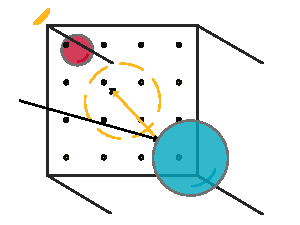
\includegraphics[width=8cm]{drawings/examples/LightIntersection.pdf}
  \caption{Example - Shadow Mesh Intersection}
  \label{fig:light-mesh-intersection}
\end{figure}

Figure~\ref{fig:light-mesh-intersection} illustrates the ray tracing algorithm
presented in this section.  The figure shows a viewing ray entering a voxel.  
The ray intersects a blue sphere.  The scene contains a single luminaire 
which results in \textbf{trace\_viewing\_rays} producing two traced images, one 
where the pixel for the viewing ray is illuminated blue and one where it is 
in shadow.  The shadow mesh generated by \textbf{trace\_light\_rays} is shown on 
the back wall of the voxel.   The closest point on the shadow mesh to the 
intersection of the light ray and voxel wall is used by 
\textbf{composite\_image} to determine if the pixel in the final image should be 
illuminated blue or in shadow.  The four closest points are highlighted with 
a yellow circle.  The closest point is the upper right hand corner of the 
highlighted vertices and is in shadow having been blocked by the red sphere.  
This results in the final image containing a shaded pixel for the represented 
viewing ray.

Figure~\ref{fig:trace}a illustrates the viewing rays as computed by
\textbf{distribute\_viewing\_rays}.  Figure~\ref{fig:trace}b illustrates the
result of all calls to \textbf{trace\_viewing\_rays} using a single ambient
light. The color of the viewing rays is set to the color of intersected objects.

\begin{figure}[!htb]
\centering
\begin{subfigure}{.49\columnwidth}
 \centering
  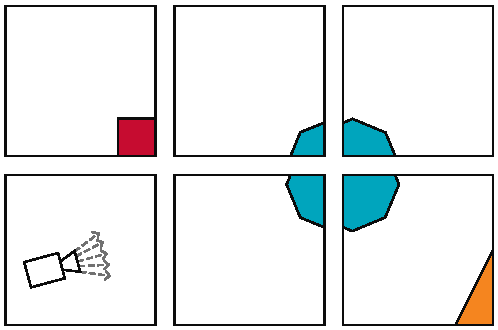
\includegraphics[width=.98\columnwidth]{drawings/examples/Trace1.pdf}
  a) Distribute Viewing Rays
\end{subfigure}
\begin{subfigure}{.49\columnwidth}
 \centering
  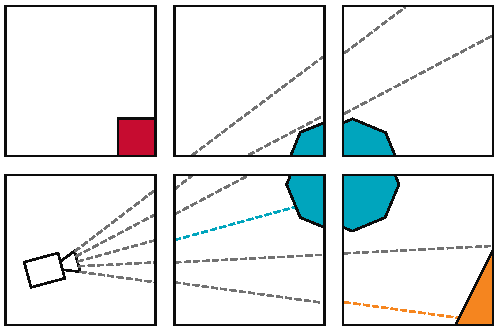
\includegraphics[width=.98\columnwidth]{drawings/examples/Trace2.pdf}
  b) Trace Viewing Rays
\end{subfigure}
\begin{flushleft}\caption{Example - Distribute and Trace Viewing Rays}{Viewing
rays are colored by the objects they intersect in the voxels of
intersection.}%
\label{fig:trace}
\end{flushleft}
\end{figure}












